\documentclass{beamer}
\usetheme{}
\usecolortheme{dolphin}           
\useinnertheme{circles}
\setbeamertemplate{itemize items}[default]
\setbeamertemplate{enumerate items}[default]
\usepackage[T1]{fontenc}
\usepackage[utf8]{inputenc}
\usepackage{lmodern}
\usepackage{amsmath}
\usepackage{booktabs} 
\usepackage{graphicx}        
\usepackage{array}
\usepackage{color}
\makeatletter
\def\zapcolorreset{\let\reset@color\relax\ignorespaces}
\def\colorrows#1{\noalign{\aftergroup\zapcolorreset#1}\ignorespaces}
\makeatother
\graphicspath{{/home/swl/Dropbox/ucd/advanced_macro/figures/}} 
\setbeamertemplate{navigation symbols}{}
\setbeamertemplate{footline}[frame number]
%--------------------------------------
\title{Real Business Cycle}
\author{School of Economics, University College Dublin}
\date{Spring 2018}
\begin{document}

%--------------------------------------
\begin{frame}
 \titlepage
\end{frame}
%--------------------------------------

%--------------------------------------
\begin{frame}
  \begin{figure}
    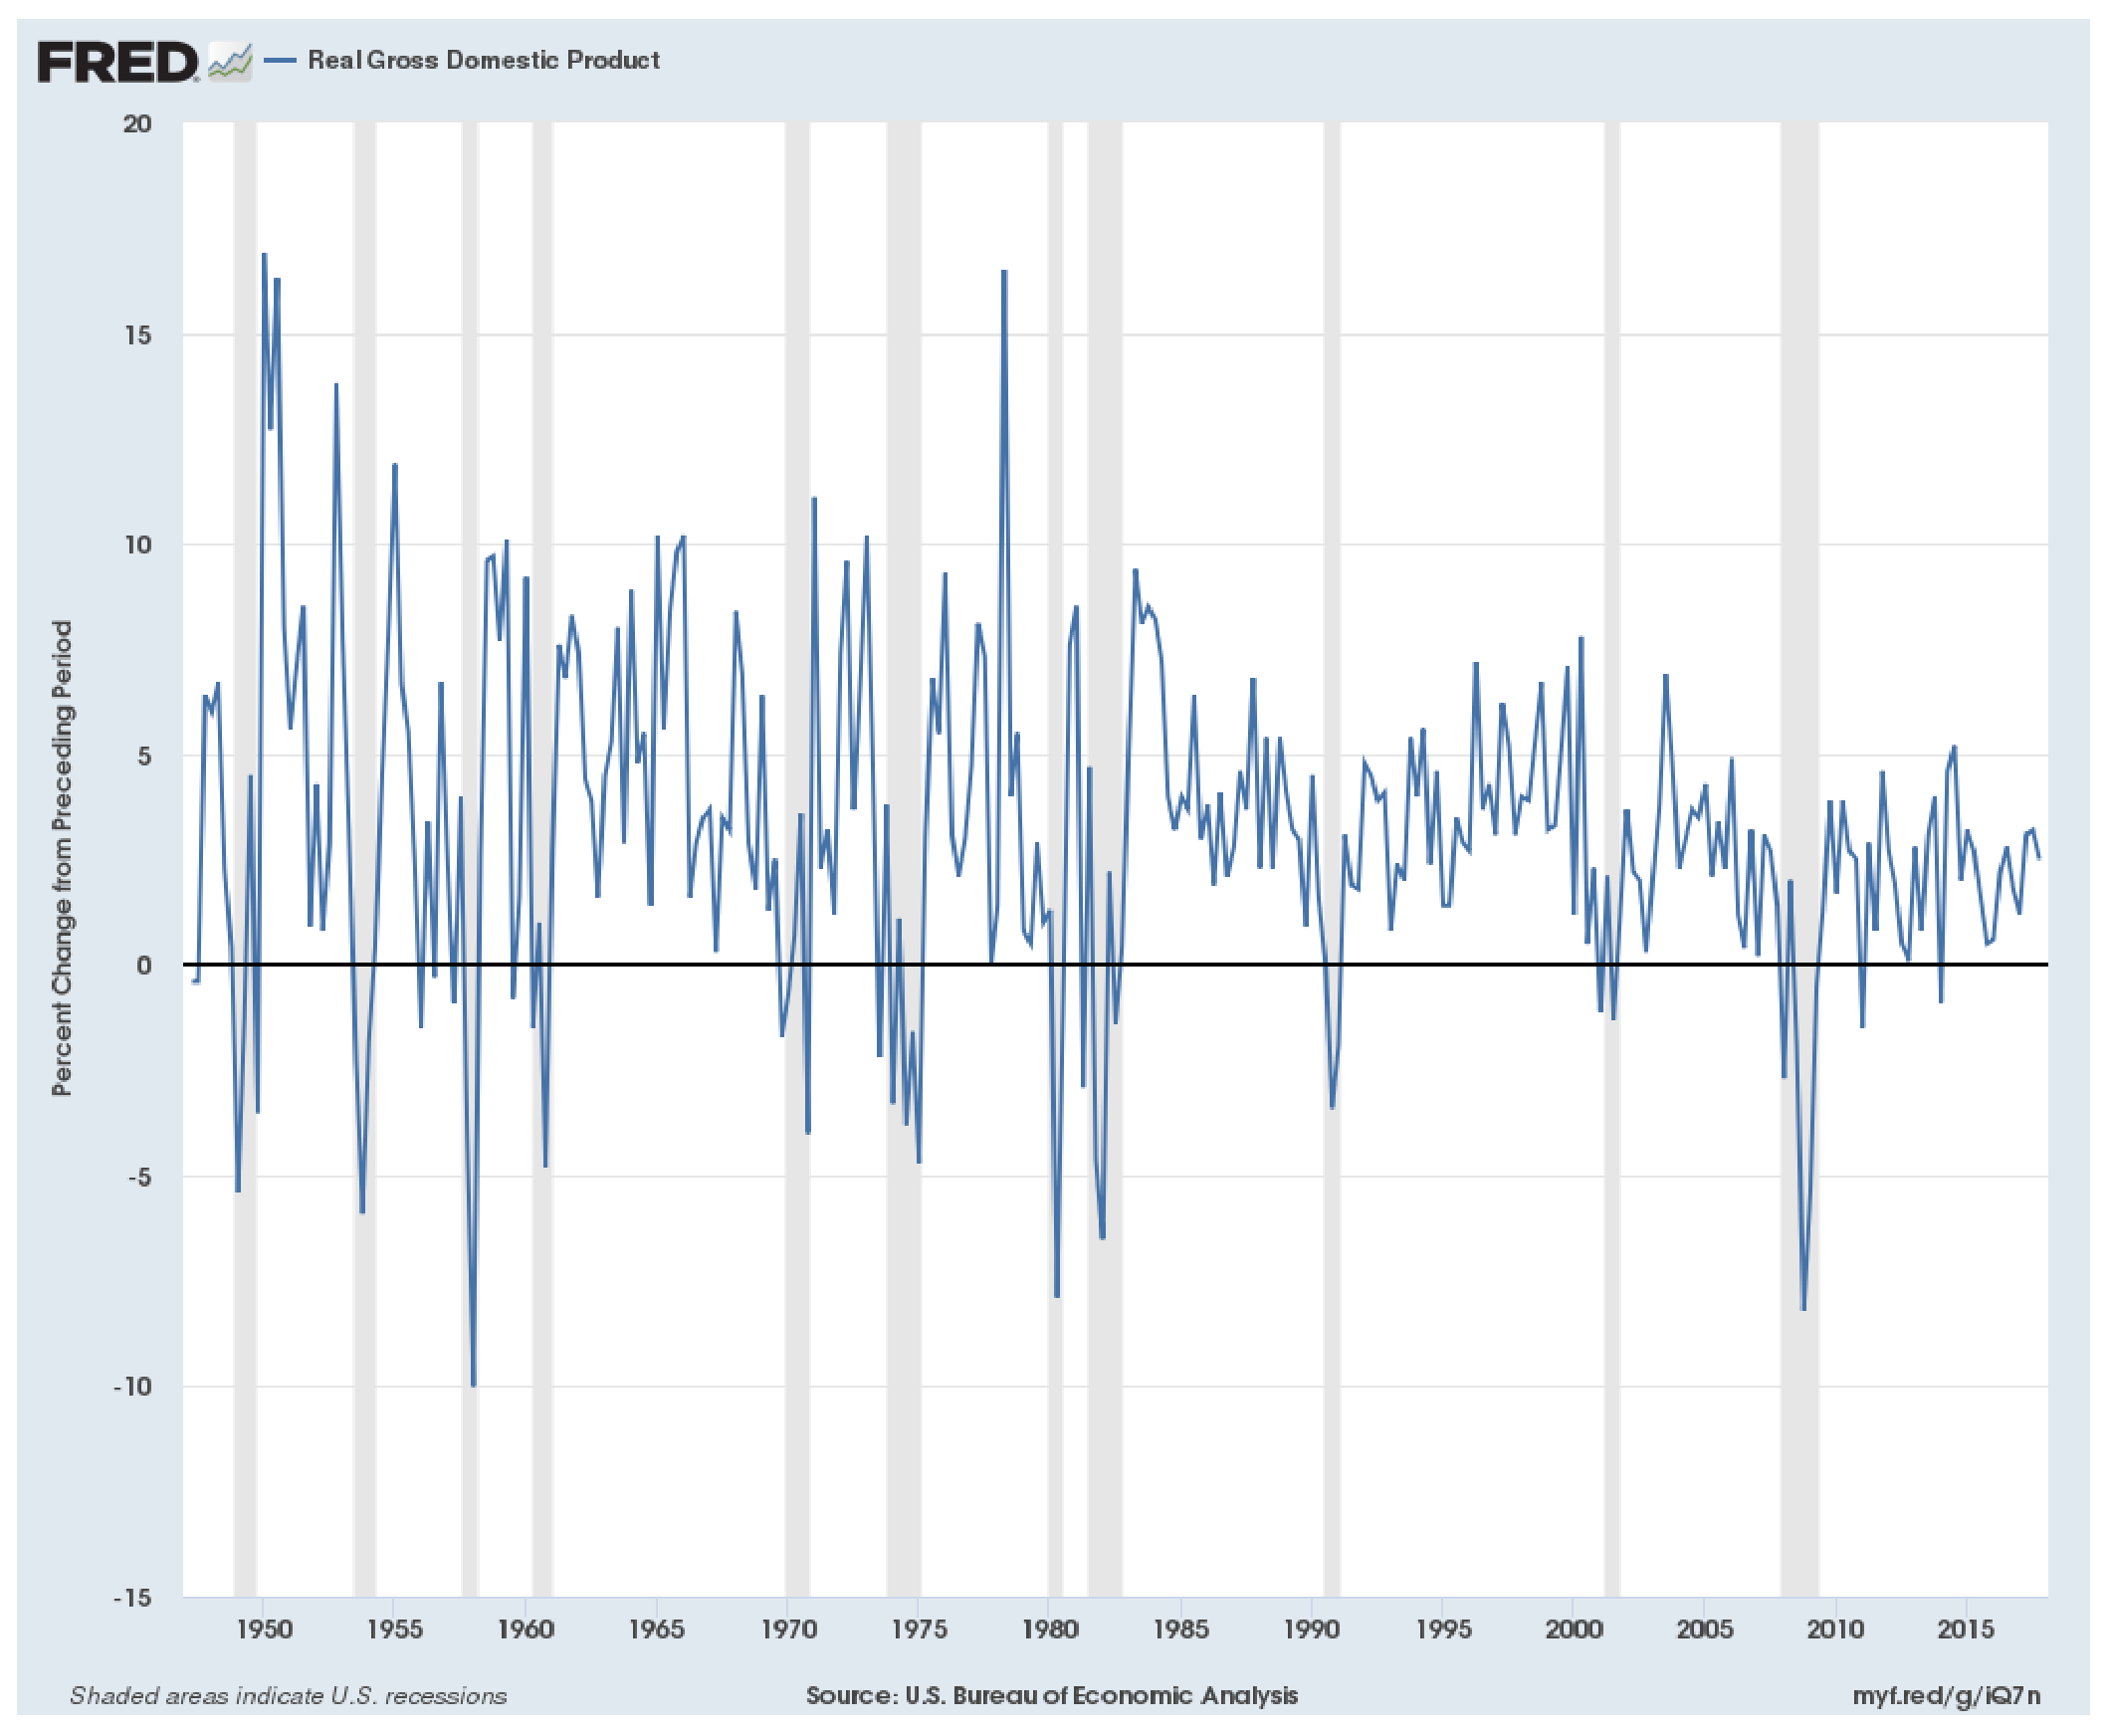
\includegraphics[scale=.25]{fred.eps}
  \end{figure}
\end{frame}
%--------------------------------------

%--------------------------------------
\begin{frame}
  \begin{figure}
    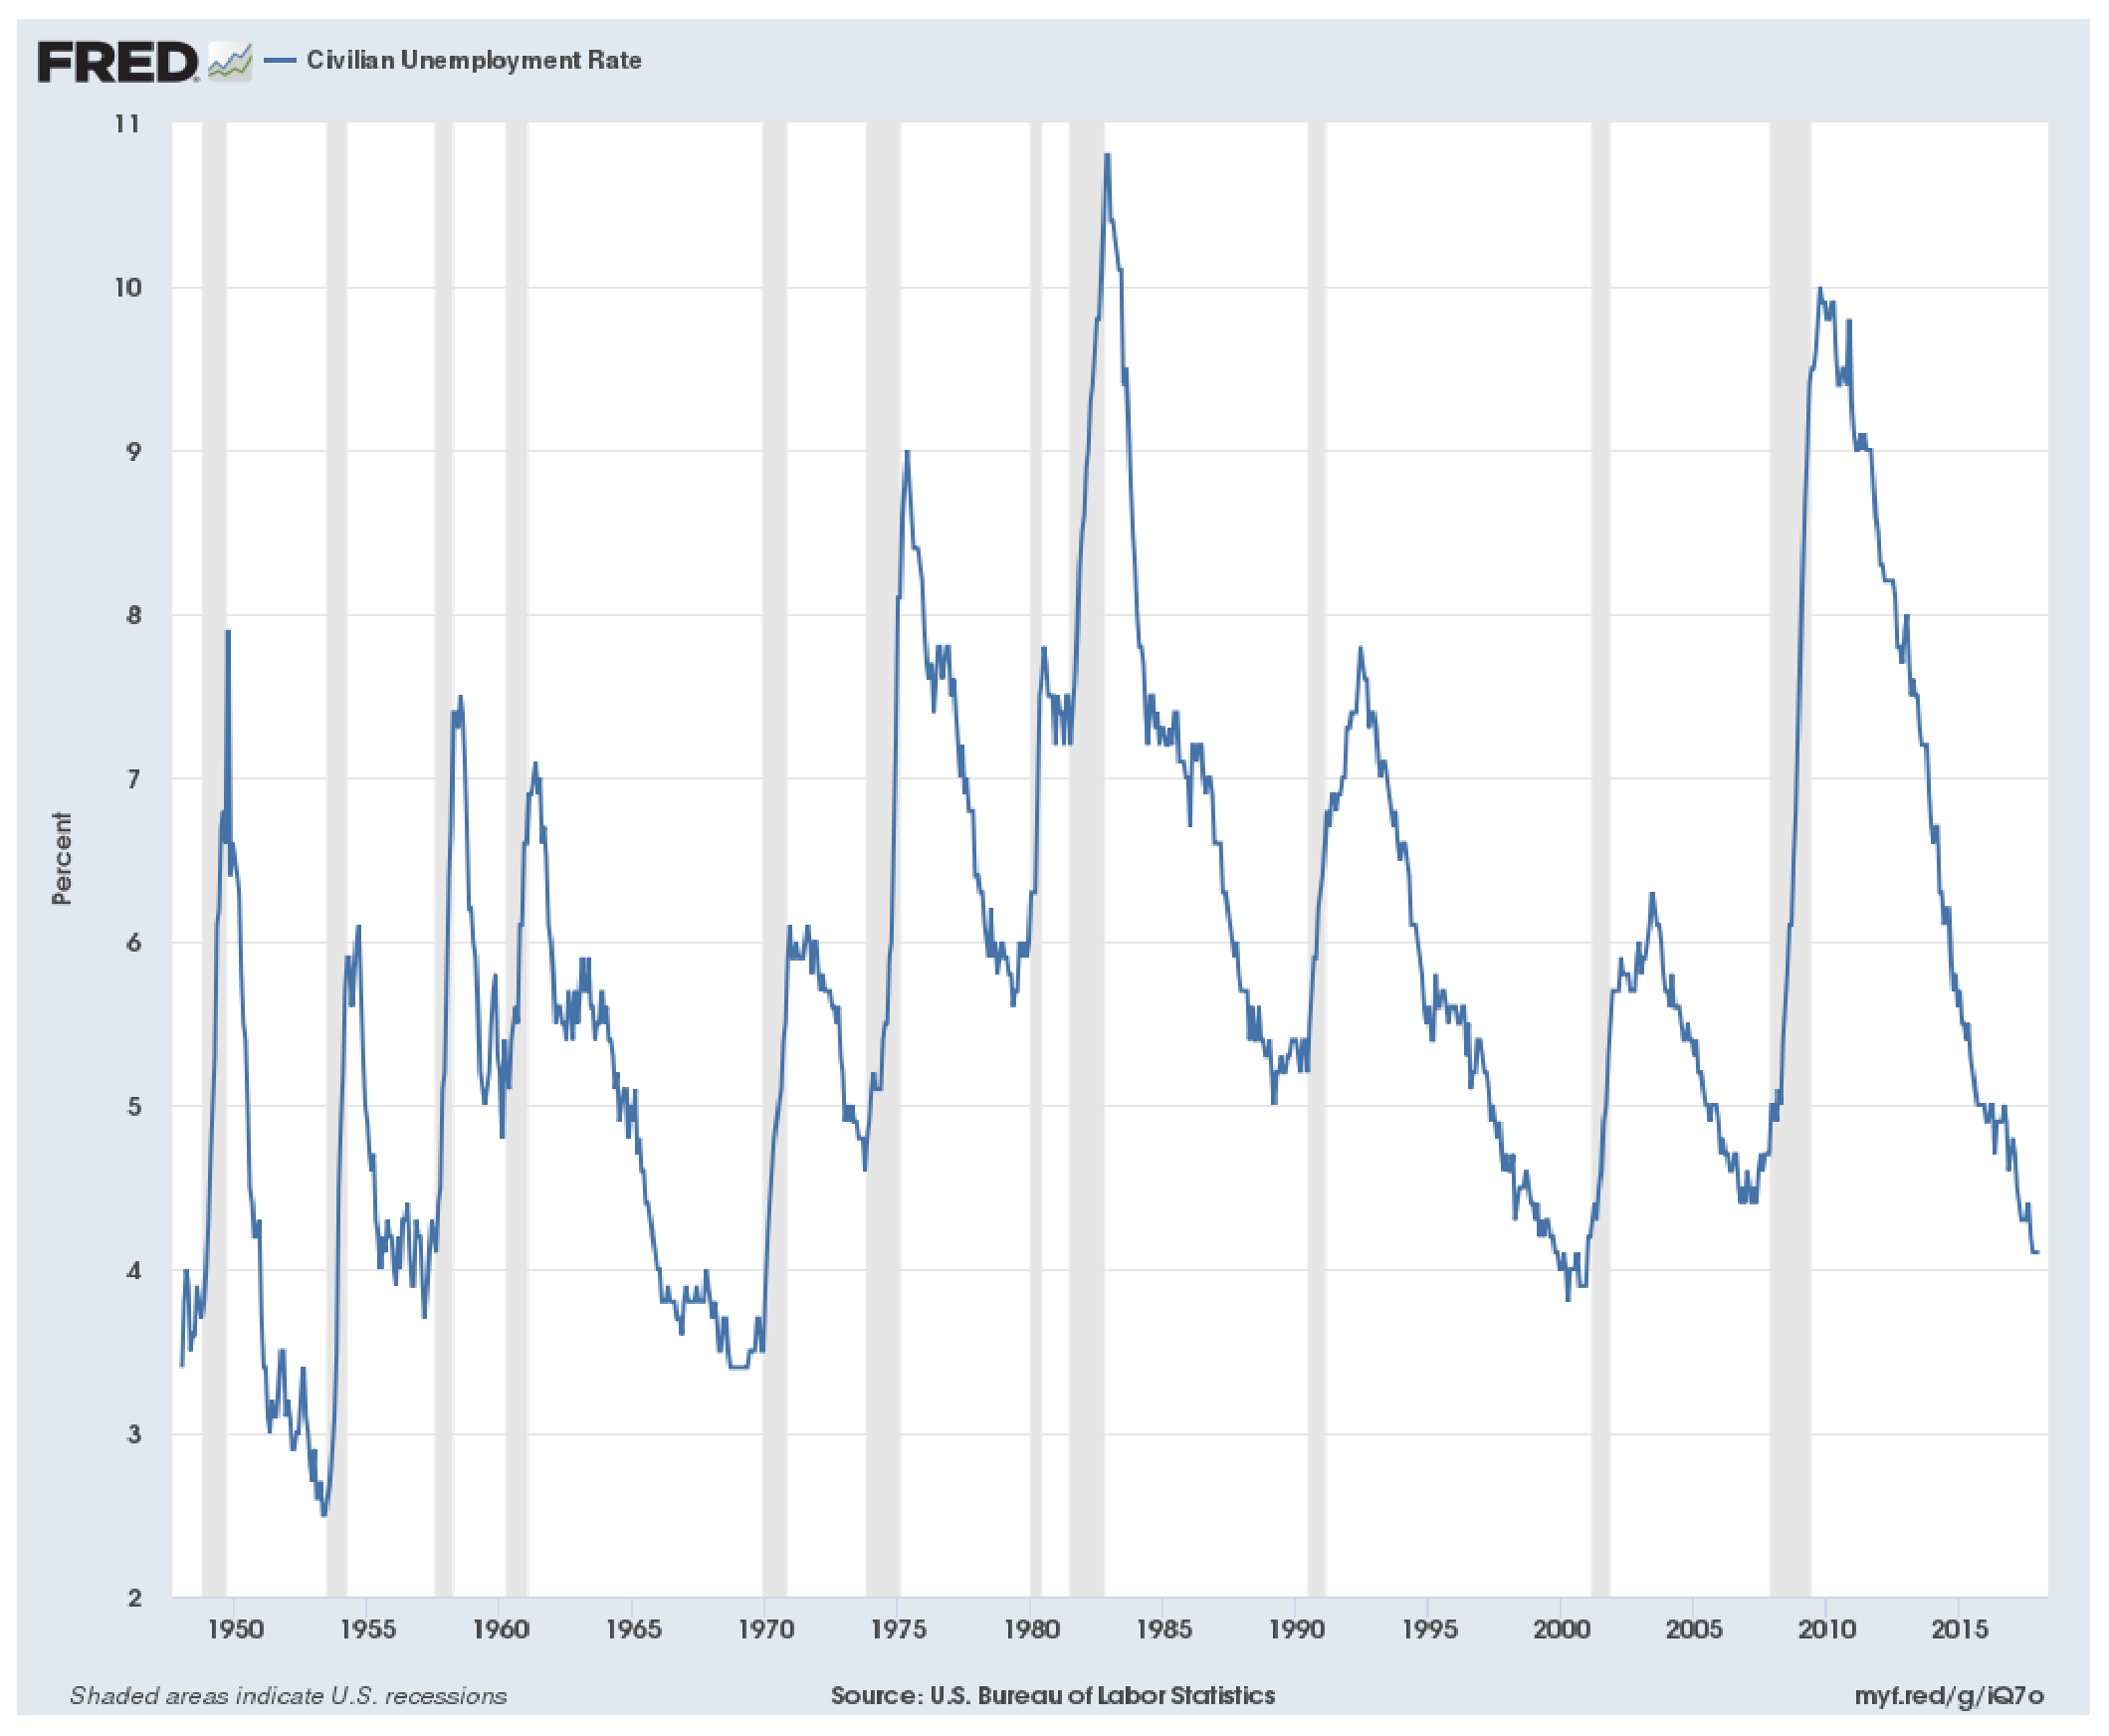
\includegraphics[scale=.25]{fred2.eps}
  \end{figure}
\end{frame}
%--------------------------------------


%--------------------------------------
\begin{frame}
  \begin{figure}
    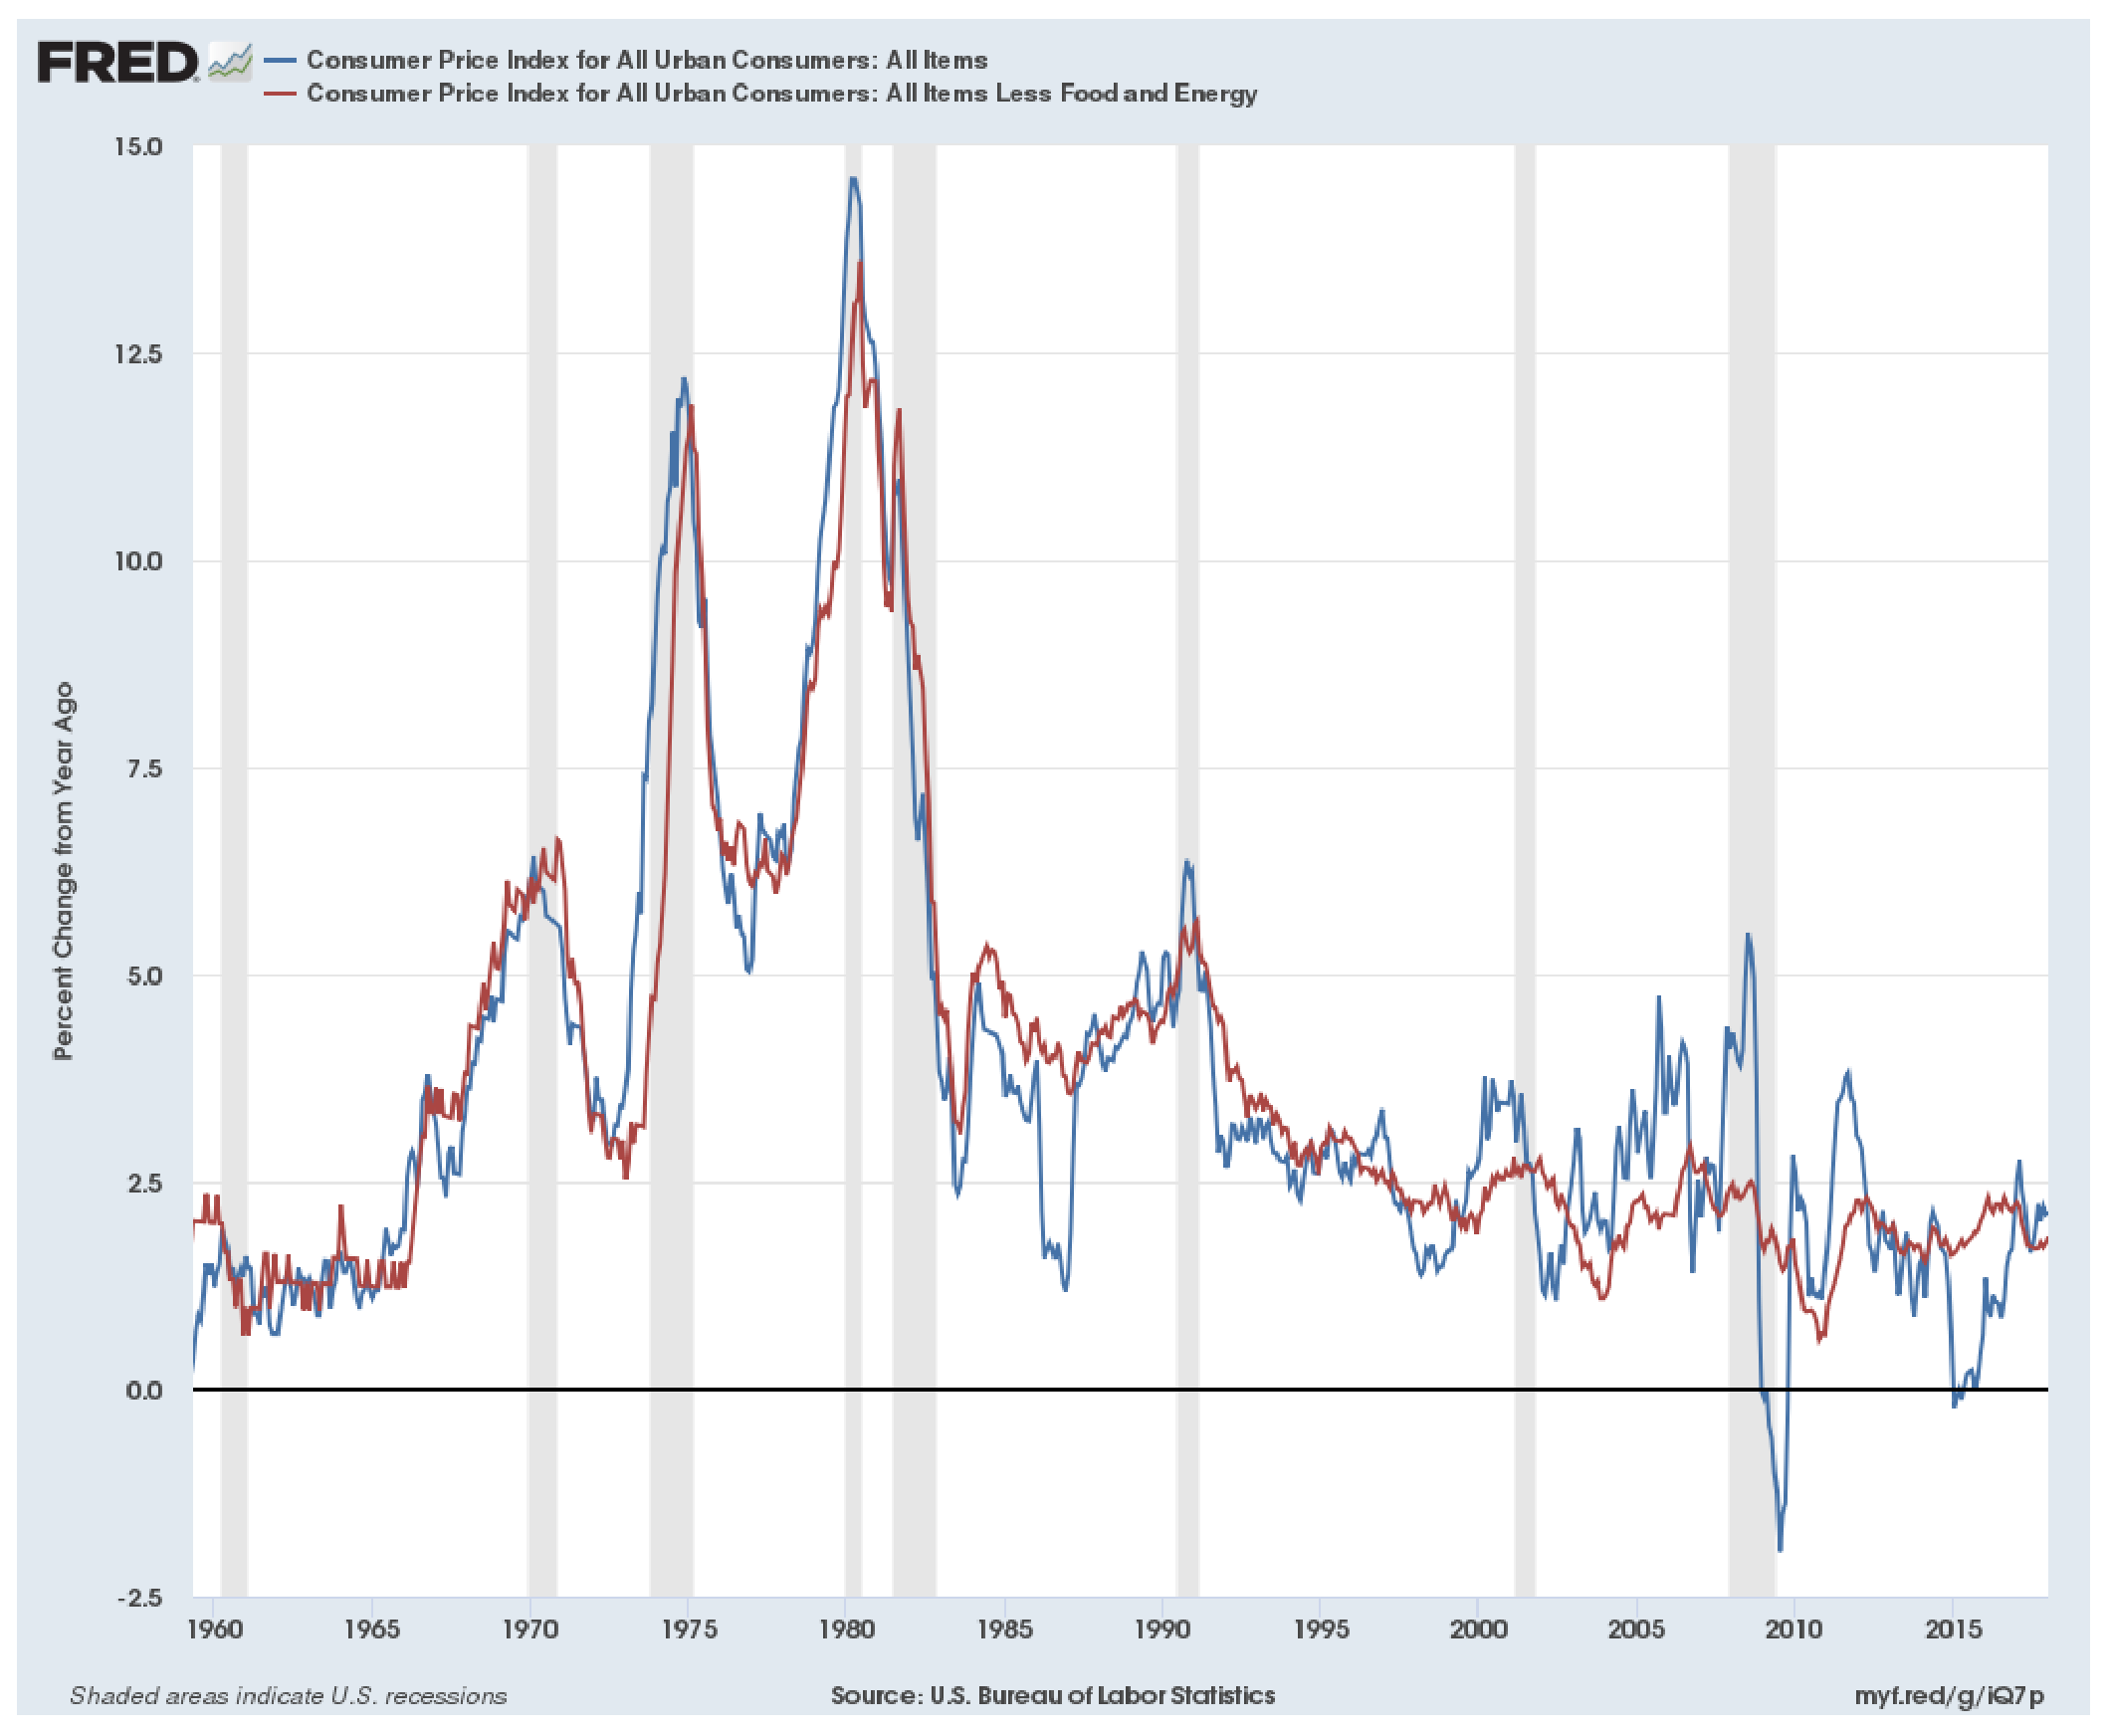
\includegraphics[scale=.25]{fred3.eps}
  \end{figure}
\end{frame}
%--------------------------------------

%--------------------------------------
\begin{frame}
  \begin{figure}
    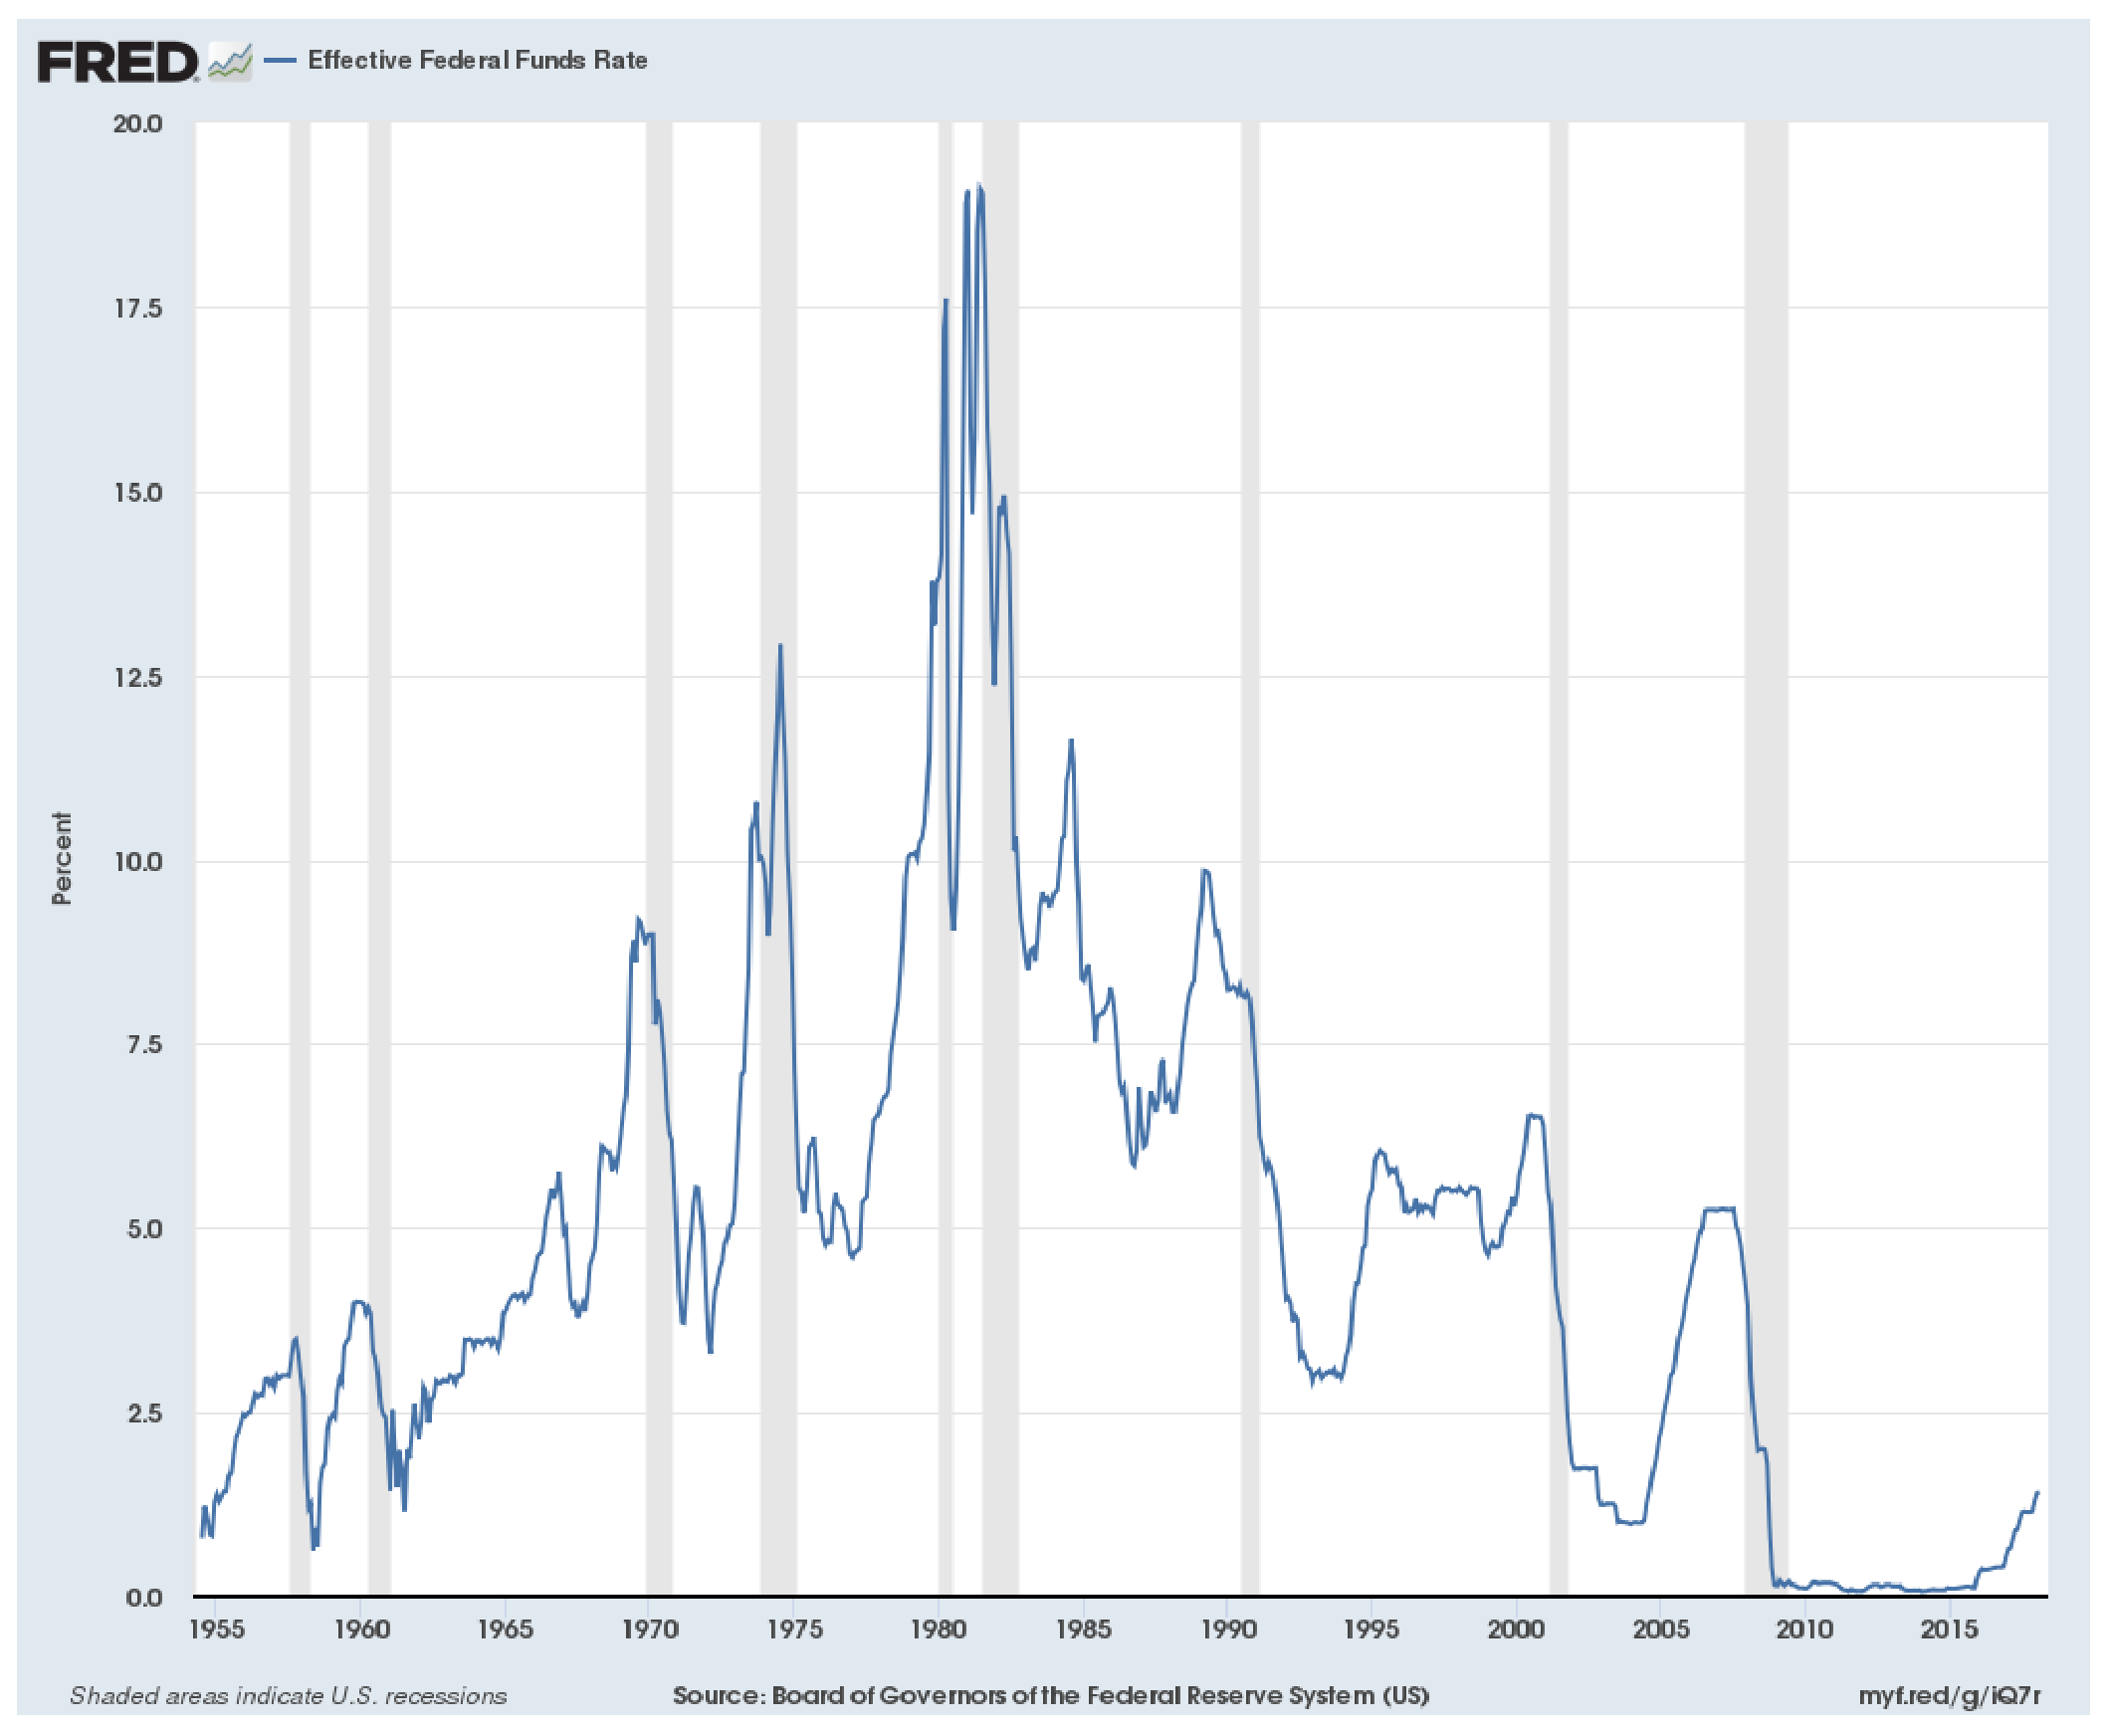
\includegraphics[scale=.25]{fred4.eps}
  \end{figure}
\end{frame}
%--------------------------------------

%--------------------------------------
\begin{frame}
  \begin{figure}
    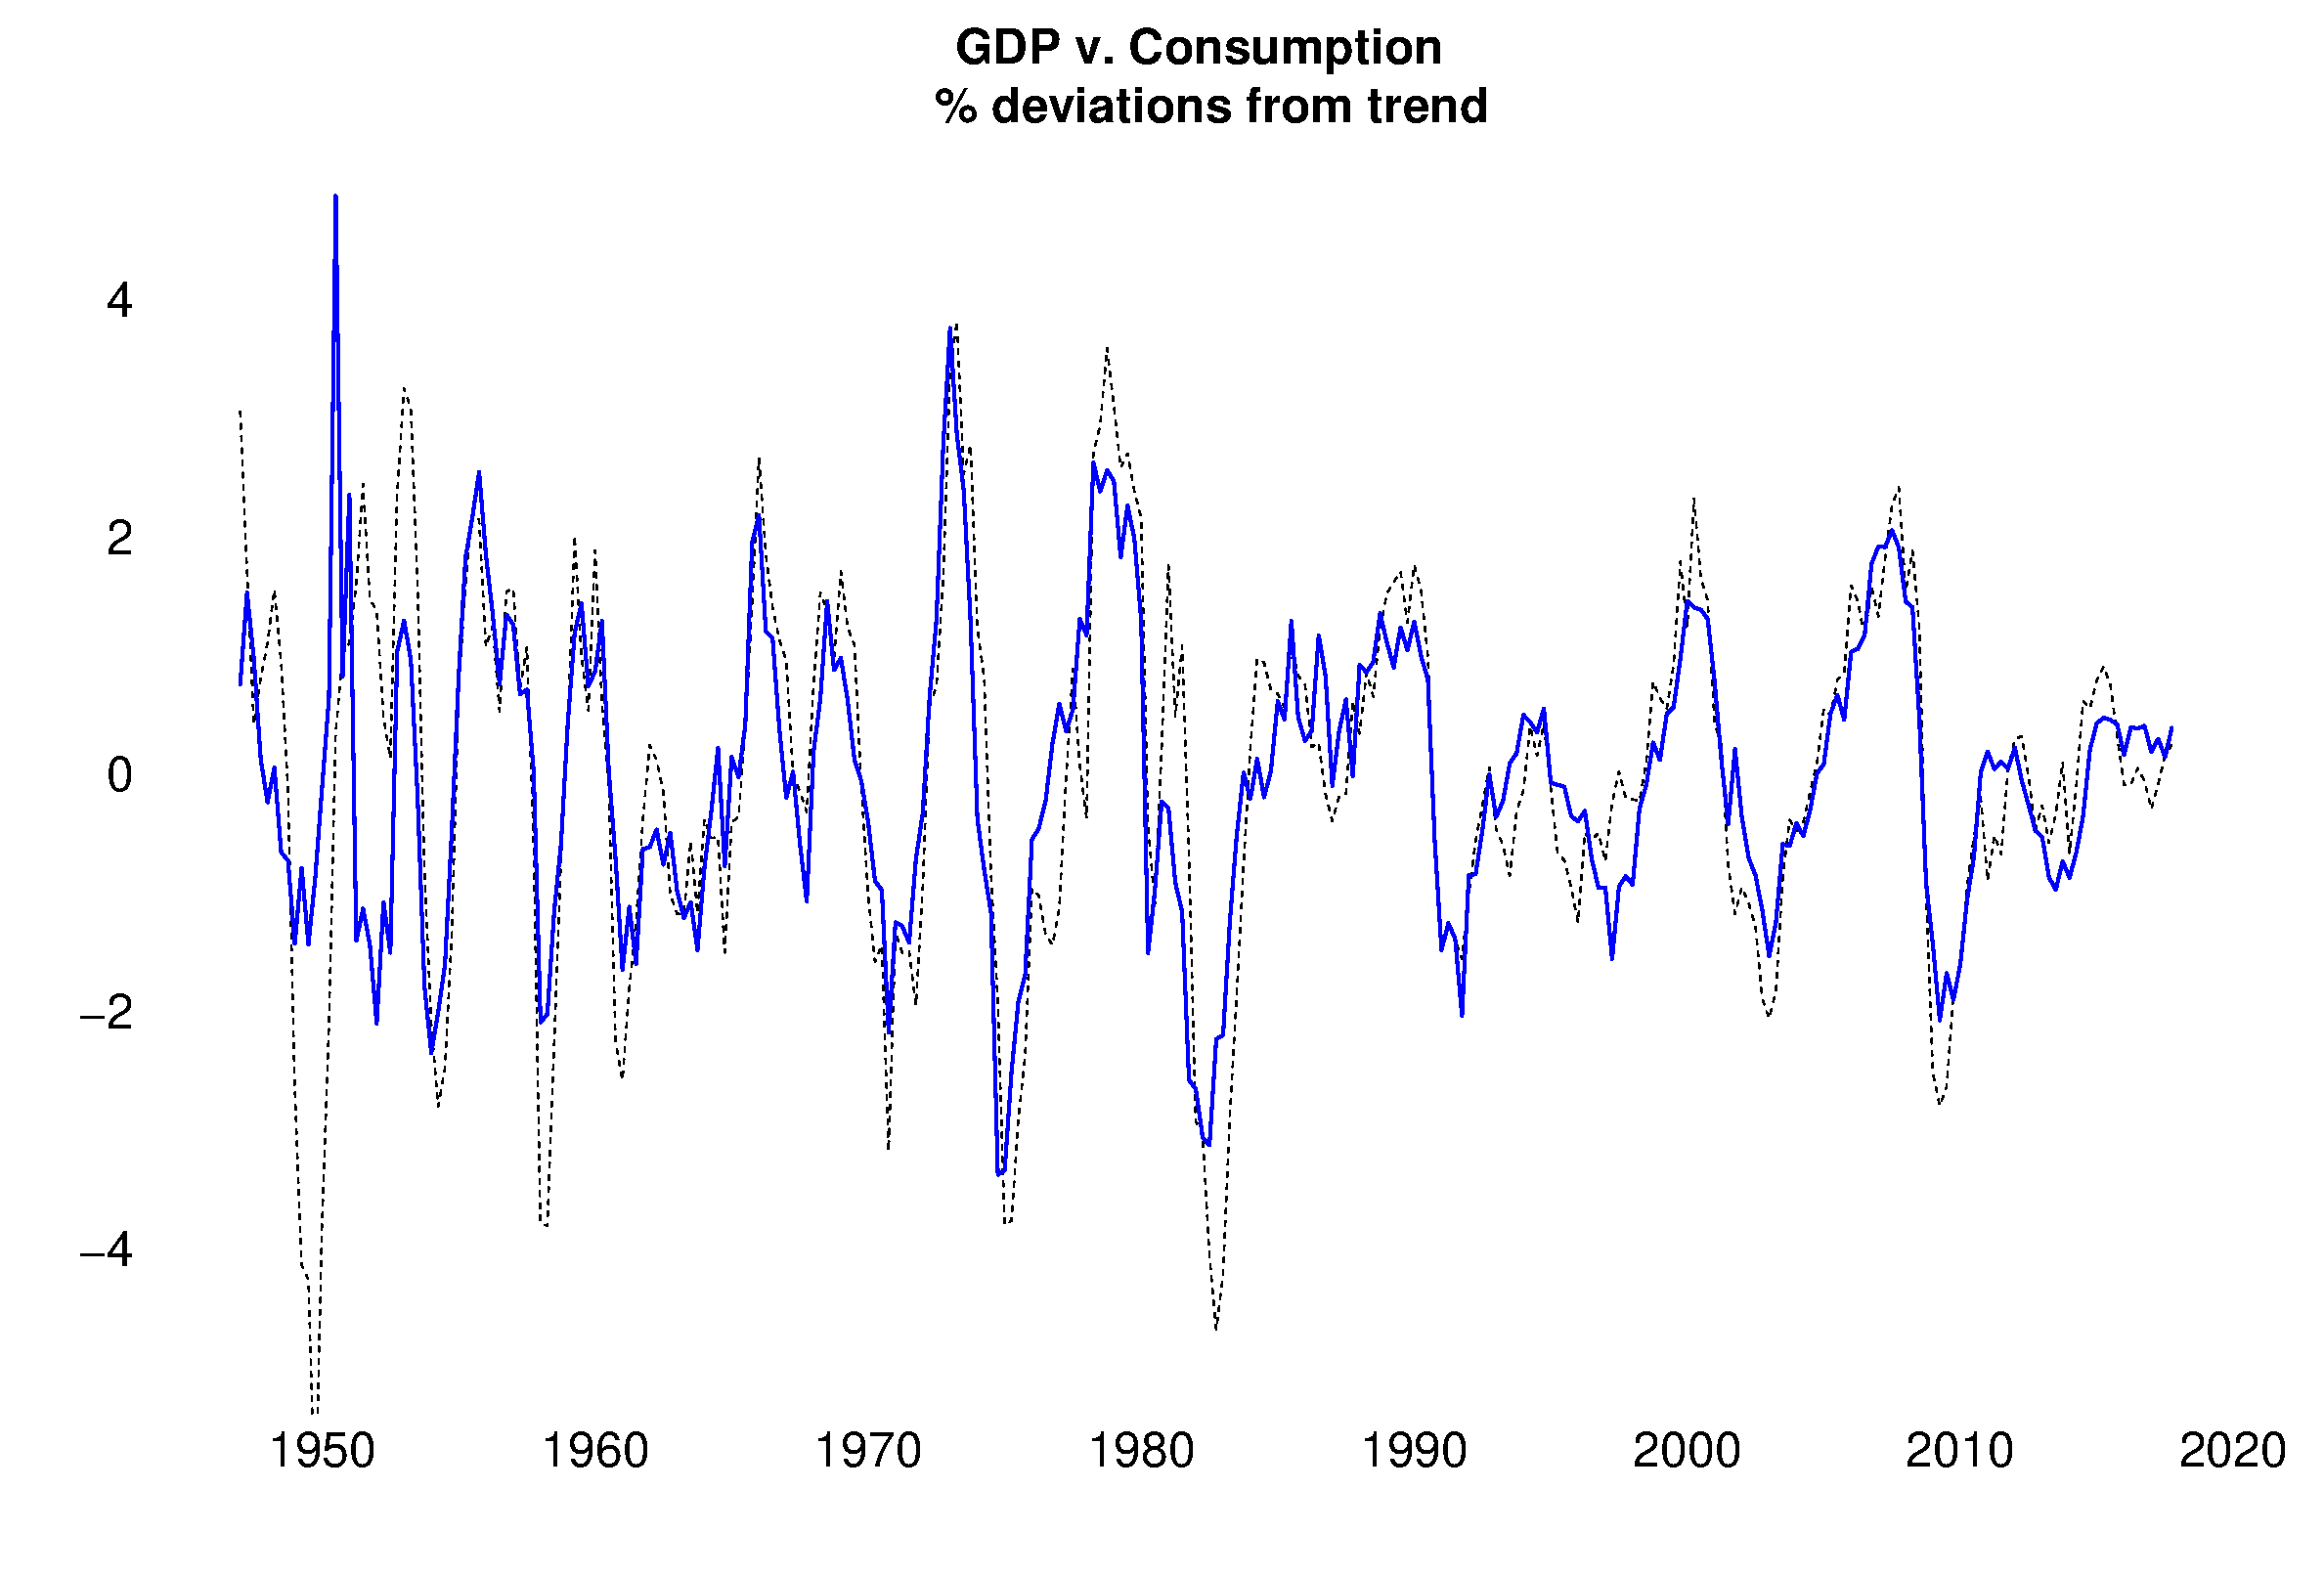
\includegraphics[scale=.25]{business_cycle.eps}
  \end{figure}
\end{frame}
%--------------------------------------

%--------------------------------------
\begin{frame}
  \begin{figure}
    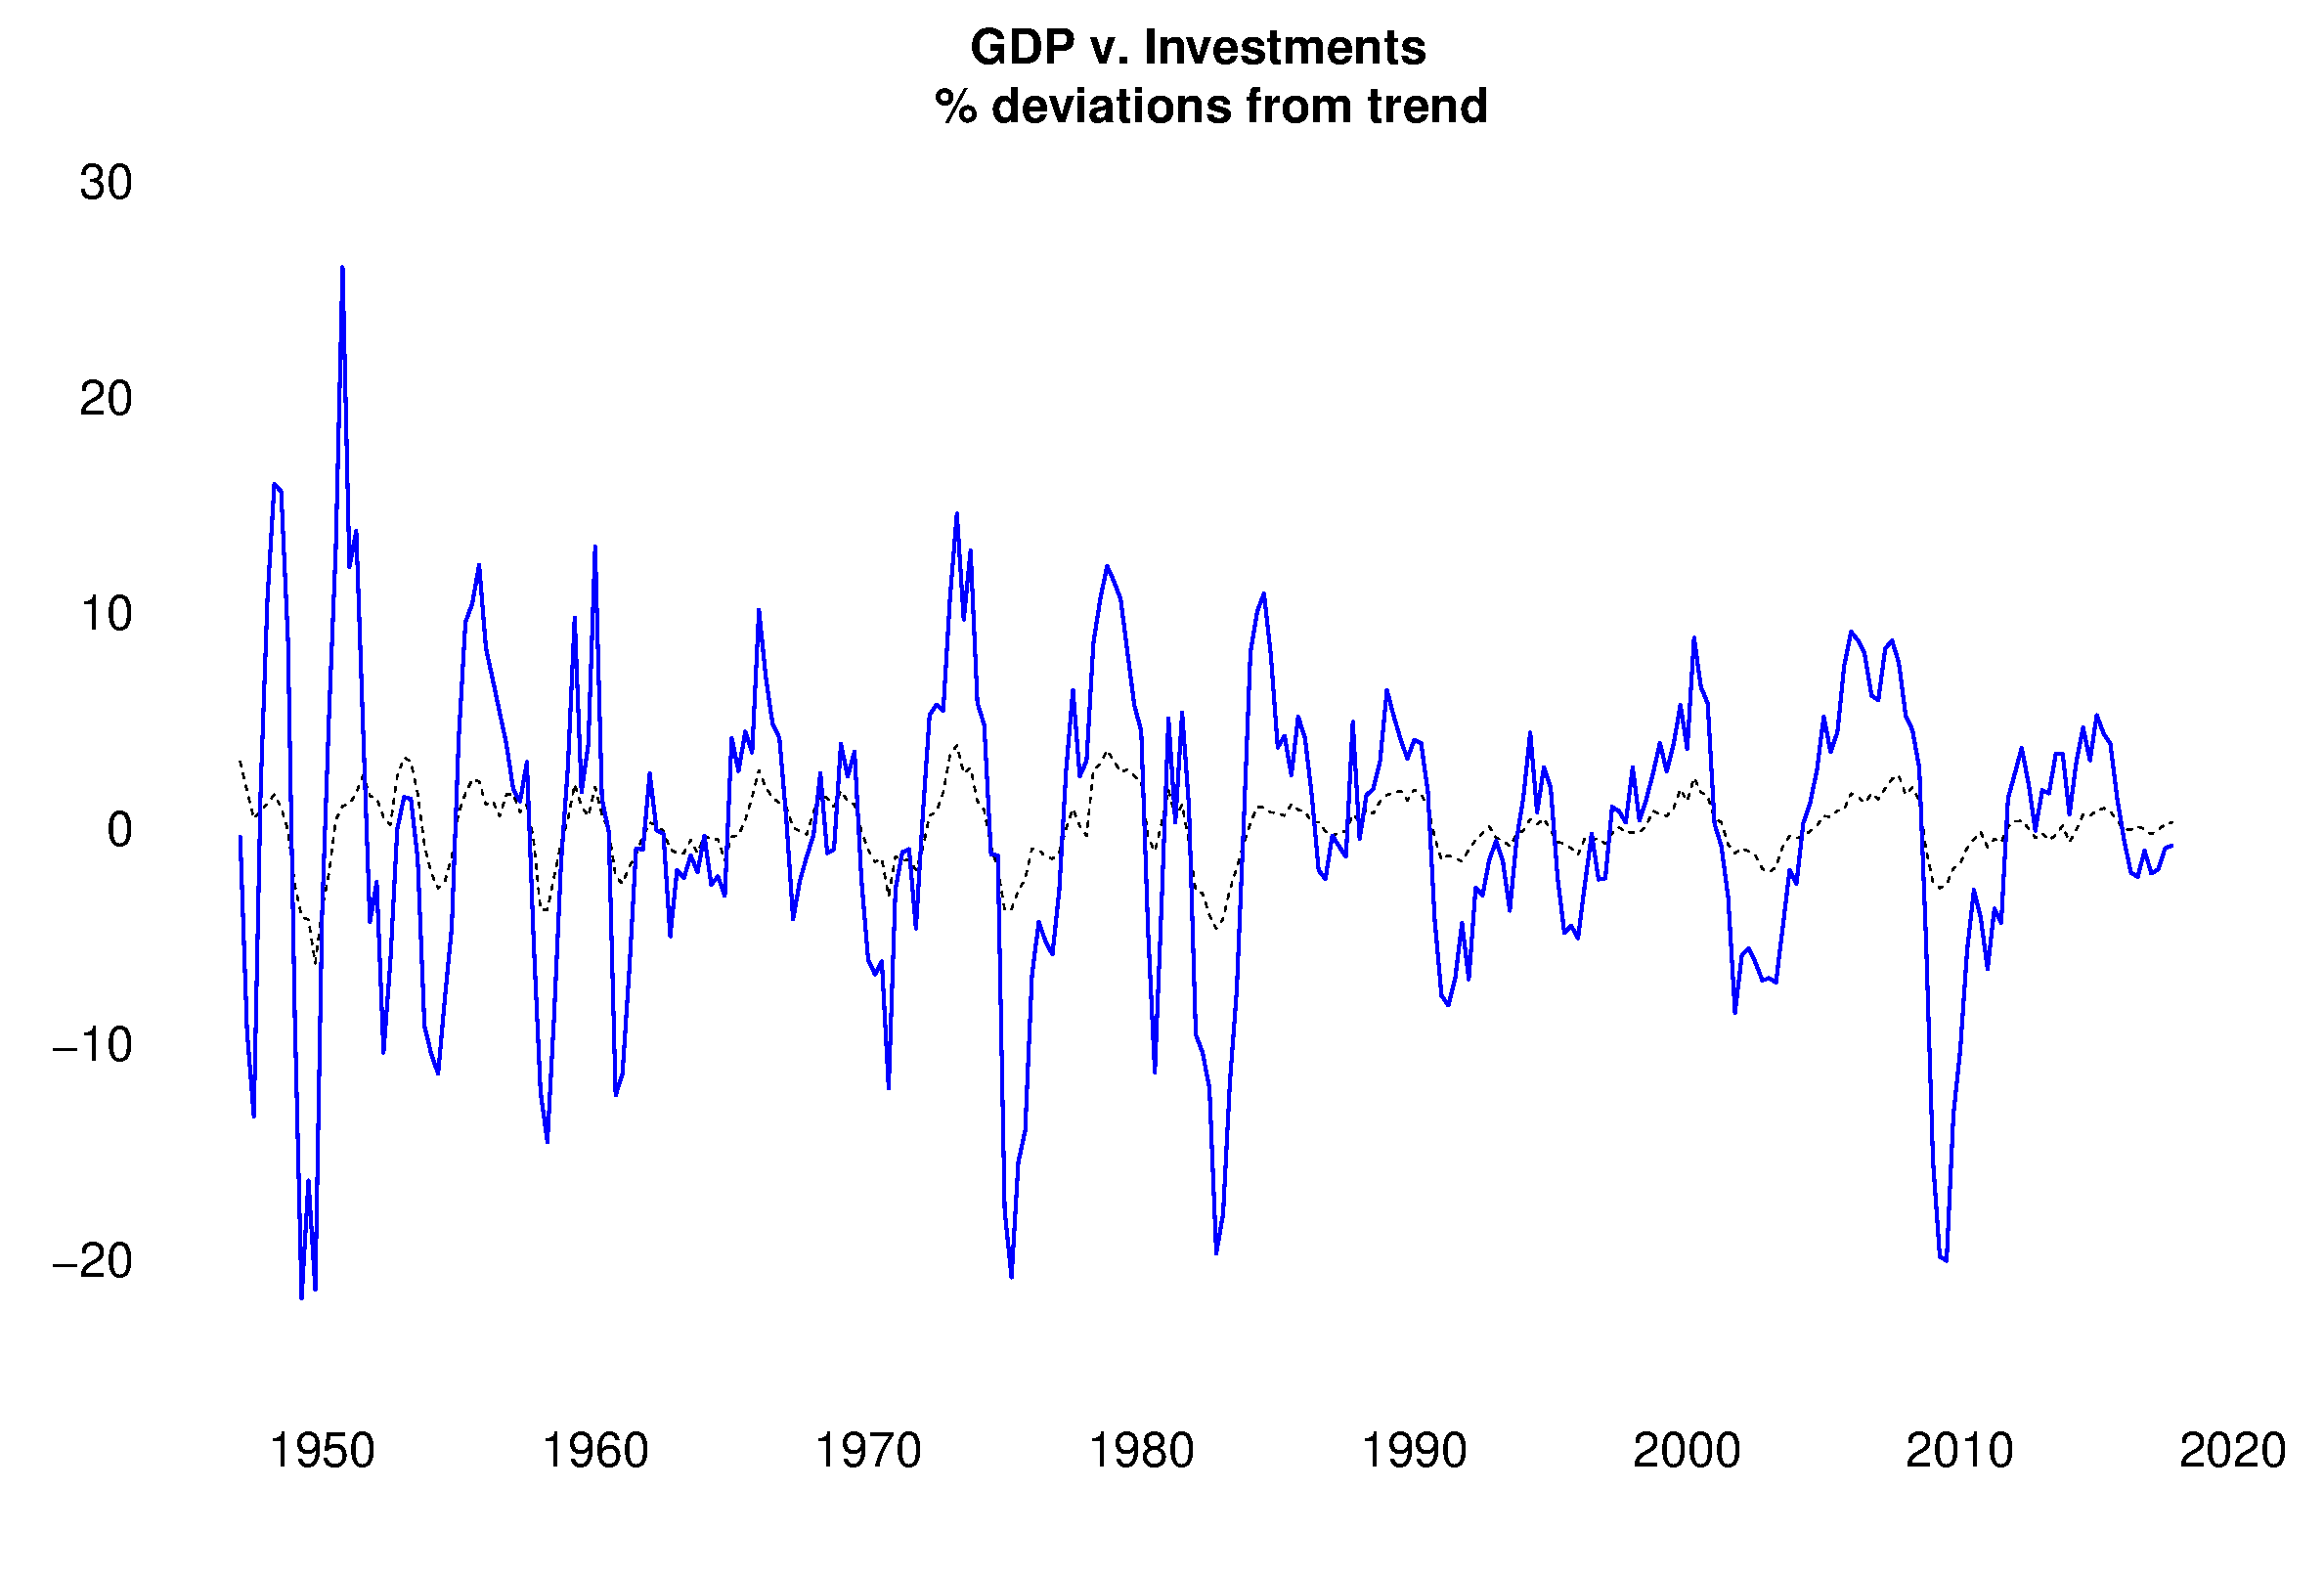
\includegraphics[scale=.25]{business_cycle2.eps}
  \end{figure}
\end{frame}
%--------------------------------------

%--------------------------------------
\begin{frame}
  \begin{figure}
    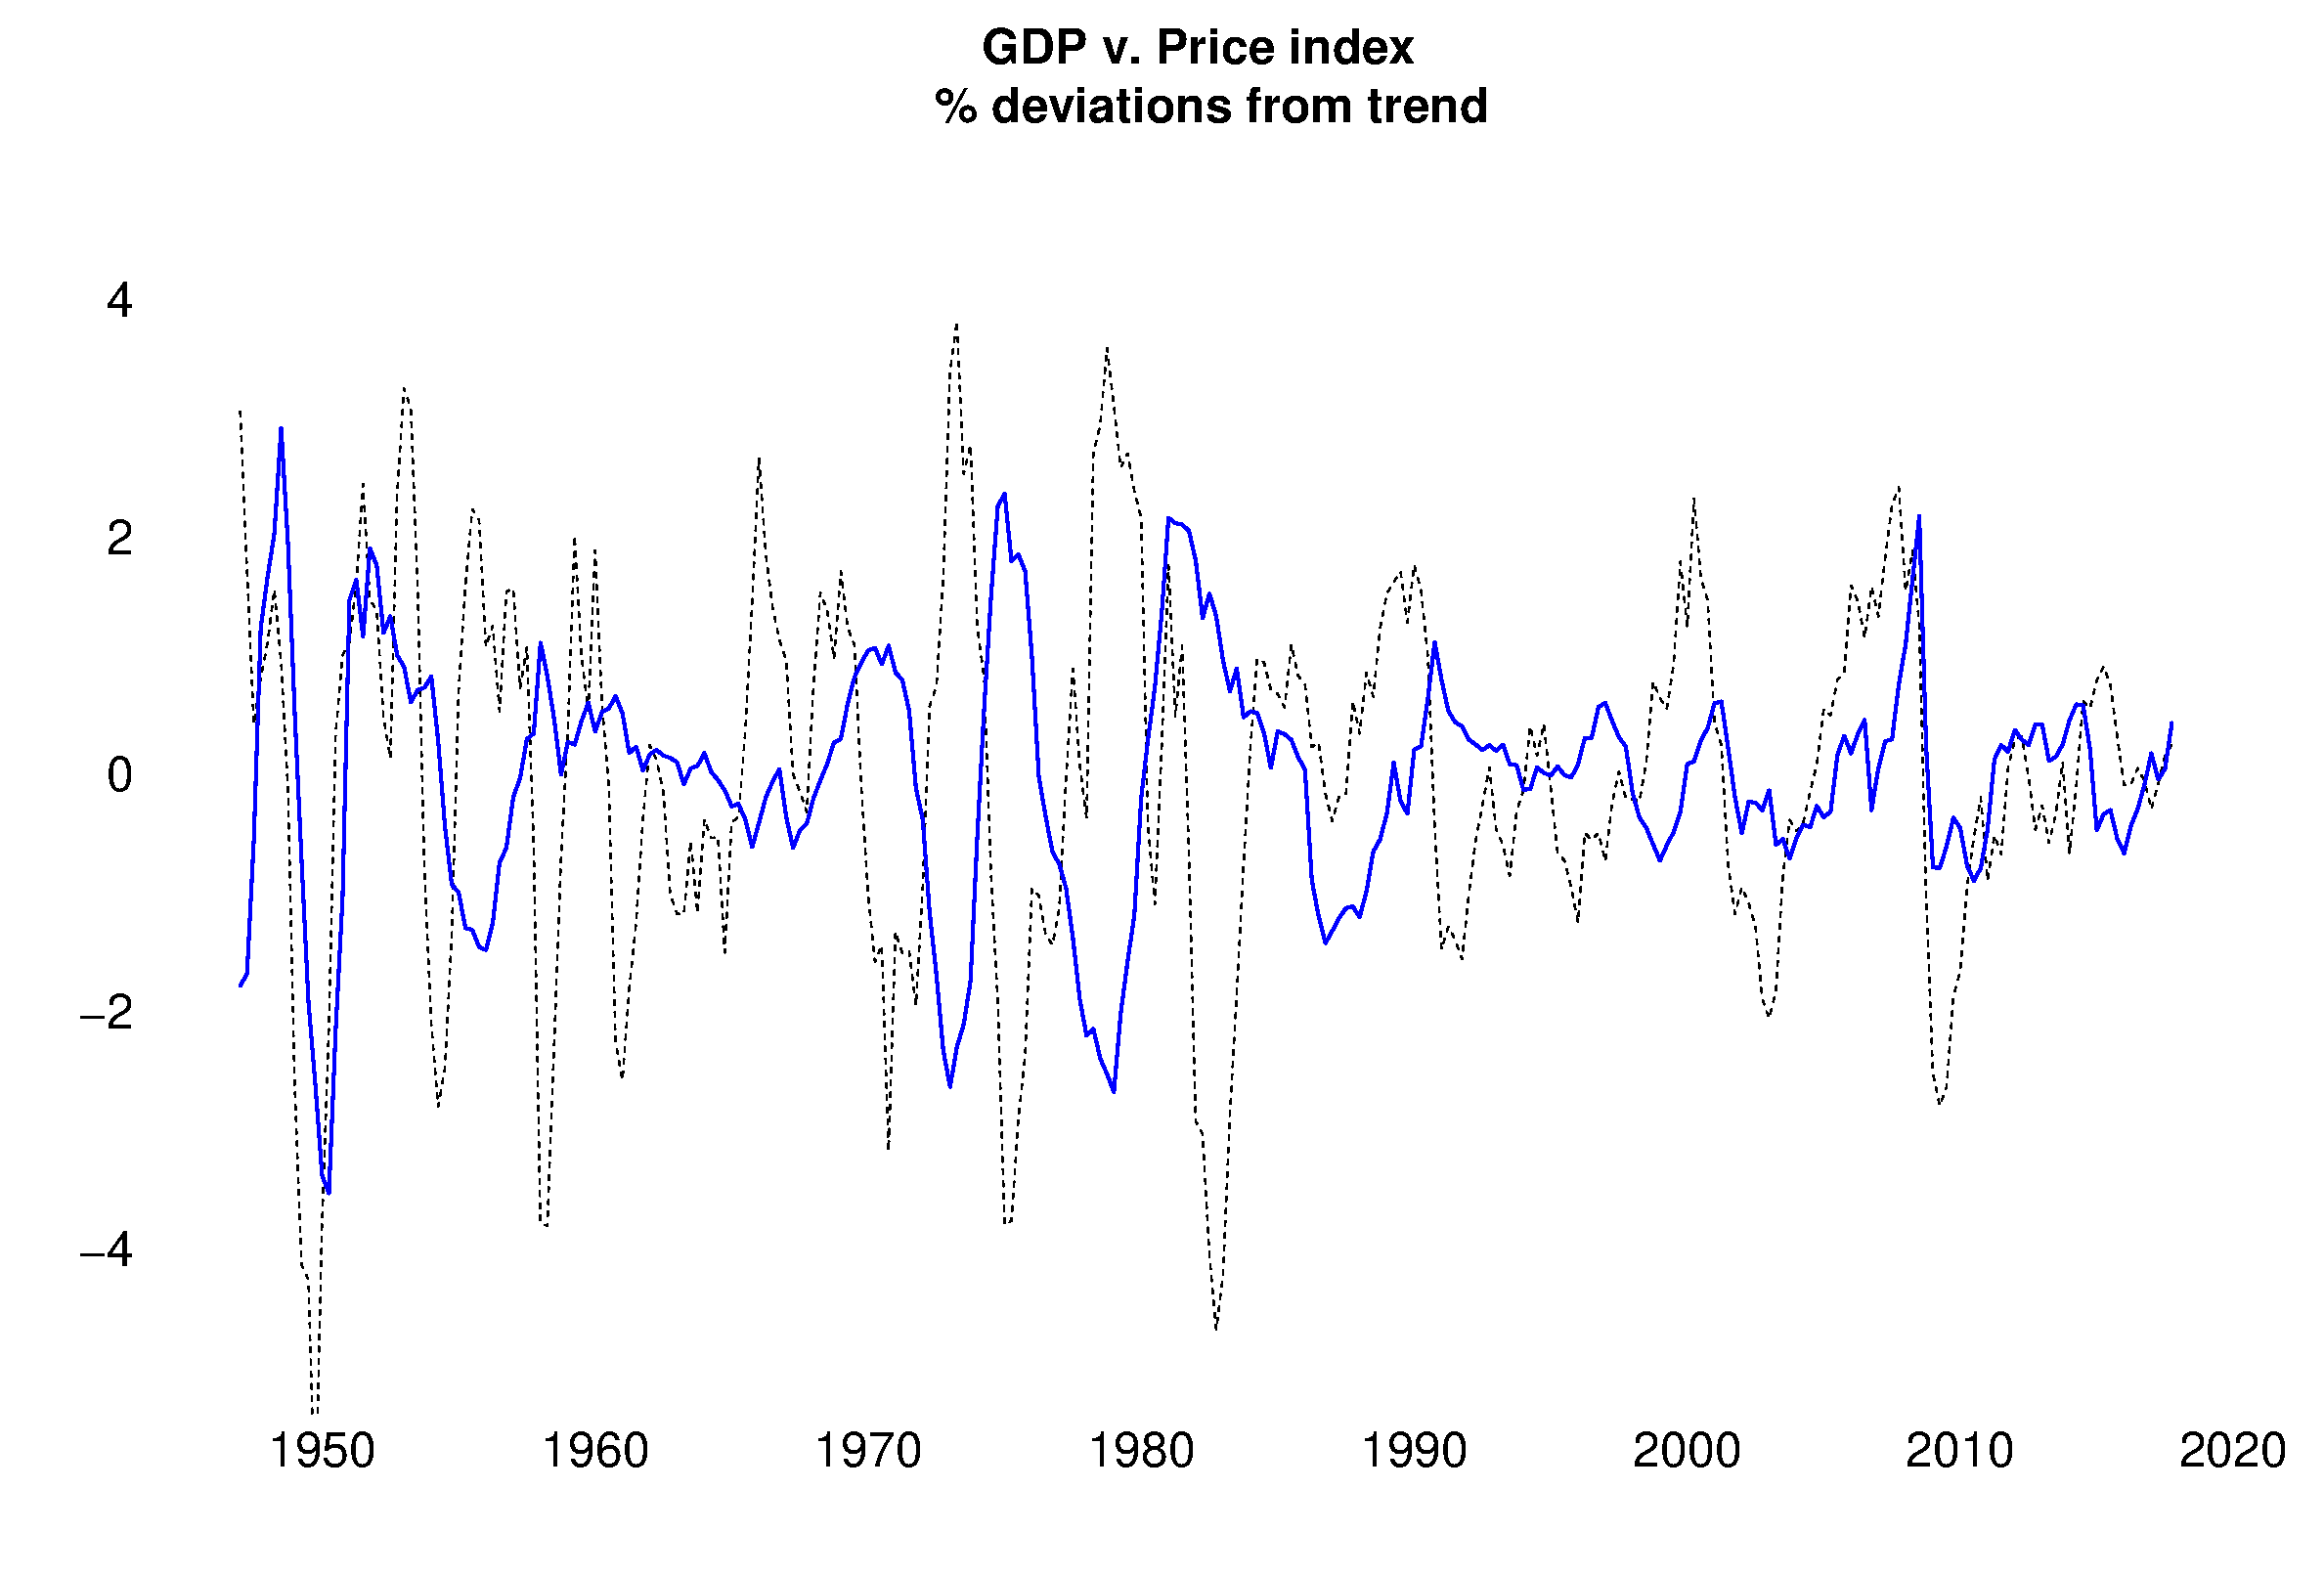
\includegraphics[scale=.25]{business_cycle3.eps}
  \end{figure}
\end{frame}
%--------------------------------------

%--------------------------------------
\begin{frame}
  \begin{figure}
    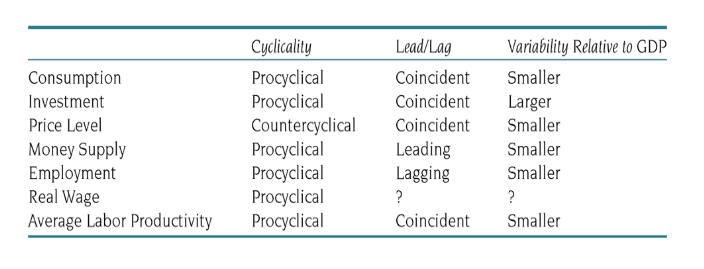
\includegraphics[scale=.8]{williamson.eps}
  \end{figure}
  Source: Williamson (1995), 'Macroeconomics'
\end{frame}
%--------------------------------------

%--------------------------------------
\begin{frame}
  \textbf{Business cycles}\\
  Economies fluctuate over time: need to explain
  \begin{enumerate}
    \item Volatility
    \item Comovements
    \item Persistence (autocorrelation)
    \item Effect of expectations on current decisions
  \end{enumerate}
  \medskip
  Two theoretical approaches 
  \begin{enumerate}
    \item Market clearing
    \item Non-market clearing
  \end{enumerate}
\end{frame}
%--------------------------------------

%--------------------------------------
\begin{frame}
  Two competing models
  \begin{enumerate}
    \item Real Business Cycle model (RBC)
    \item New-Keynesian model (NK)
  \end{enumerate}
  \medskip
  Similarities
  \begin{itemize}
    \item Dynamic general equilibrium
    \item Stochastic shocks
    \item Forward looking expectations
  \end{itemize}
  \medskip
  Main difference concerns information and prices
  \begin{itemize}
    \item RBC: Complete and flexible 
    \item NK: Incomplete and sticky
  \end{itemize}
\end{frame}
%--------------------------------------

%--------------------------------------
\begin{frame}
  \textbf{Real Business Cycle model}\\
  \begin{enumerate}
    \item Take Swan-Solow growth model
    \item Insert (1) into dynamic optimisation framework
    \begin{itemize}
      \item No more constant savings rate
    \end{itemize}
    \item Add shocks to total factor productivity ($A$)
    \begin{itemize}
      \item Include uncertainty about shocks
    \end{itemize}
    \item Add leisure to account for changes in hours of work
  \end{enumerate}
\end{frame}
%--------------------------------------

%--------------------------------------
\begin{frame}
  Why real?\\
  \medskip
  Equilibrium is about
  \begin{itemize}
    \item Household preferences
    \item Technology used by firms
    \item Government policy decisions
  \end{itemize}
  \medskip
  These are \textbf{real} factors
\end{frame}
%--------------------------------------

%--------------------------------------
\begin{frame}
  Recap: \textbf{Swan-Solow model}
  \begin{align}
    Y_t &= A_tK_t^{\alpha}N_t^{1-\alpha}\\
    K_t &= (1+\delta)K_{t-1} + I_t\\
    I_t &= sY_t\\
    N_t &= (1+n)N_{t-1}\\
    A_t &= (1+m)A_{t-1}\\
    Y_t &\equiv C_t + I_t
  \end{align}
  \begin{align*}
    0<\alpha<1, \delta>0, 0<s<1
  \end{align*}
\end{frame}
%--------------------------------------

%--------------------------------------
\begin{frame}
  Model's fundamental mechanism: shocks to Total Factor Productivity (TFP)
  \begin{itemize}
    \item Recall positive correlation between GDP and productivity
  \end{itemize}
  \medskip
  Major result: Fluctuations as an equilibrium outcome
  \begin{itemize}
    \item Work harder when productivity is high: wages increase as labour becomes more productive
    \item Save more when productivity is high: interest rates increase as capital becomes more productive
  \end{itemize}
  \medskip
  Fluctuations in economy are not that bad
\end{frame}
%--------------------------------------


%--------------------------------------
\begin{frame}
  \textbf{Real Business Cycle model} assumes
  \begin{enumerate}
    \item Perfectly functioning competitive markets
    \item Rational expectations
  \end{enumerate}
  \medskip
  Outcomes generated by decentralized decisions of firms and households: can be replicated as solution to a social planner problem who want so maximise
 \begin{align}
  E_t \left[\sum^{\infty}_{i=0} \beta^i(U(C_{t+i})-V(N_{t+i})) \right]
 \end{align}
 $C_t$ is consumption\\
 $N_t$ hours worked\\
 $\beta$ is the household's rate of time preference 
\begin{align}
  U(C_t)-V(N_t)=\frac{C_t^{1-\eta}}{1-\eta}-\nu N_t
\end{align}
\end{frame}
%--------------------------------------

%--------------------------------------
\begin{frame}
 \textbf{Economic constraints}
\begin{align}
  Y_t &= C_t + I_t = A_tK^\alpha_{t-1}N^{1-\alpha}_t\\
  K_t &= I_t + (1-\delta)K_{t-1}
\end{align}
  \textbf{Technology process}  $A_t$ is usually a log-linear AR(1) process
   \begin{itemize}
    \item For simplicity assume that $A_t$ does not trend over time: economy has average growth rate of zero.
  \end{itemize}
 \begin{align}
  log\; A_t= (1-\rho) \;log\; A^* + \rho\; log\; A_{t-1} + \epsilon_t
\end{align}
$A^*$ indicates the steady-state for technology.
\end{frame}
%--------------------------------------

%--------------------------------------
\begin{frame}
  \textbf{Criticism}\\
  There is some critique on the RBC model specifically concerning
  \begin{enumerate}
    \item Assumption of perfect markets and rational expectations
    \item Role of monetary and fiscal policy
    \item Role of technology shocks
  \end{enumerate}  
\end{frame}
%--------------------------------------

%--------------------------------------
\begin{frame}
  \textbf{Perfect markets and rational expectations}\\  
  \begin{itemize}
    \item  Can economy be characterized as a perfectly competitive market equilibrium solution describing the behaviour of a set of
completely optimizing rational agents?
     \item Markets are not always competitive; people not always rational in economic decisions
  \end{itemize}
  \medskip
  RBC model a benchmark: compare with more complicated models
  \begin{itemize}
    \item Are market imperfections such as sticky price crucial to understanding macroeconomic fluctuations?
    \item Can account for imperfect competition
  \end{itemize}
\end{frame}
%--------------------------------------

%--------------------------------------
\begin{frame}
  \textbf{Monetary \& fiscal policy}\\
   \begin{itemize}
     \item RBC exhibits complete monetary neutrality
     \item Including government spending, model would exhibit Ricardian equivalence
   \end{itemize}
   \medskip
    Most modern RBC models include mechanisms allowing for monetary/fiscal policy to have Keynesian effects
  \begin{itemize}
    \item e.g. most DGSE models include sticky prices/wages; leads to real effects for monetary policy
  \end{itemize}
\end{frame}
%--------------------------------------

%--------------------------------------
\begin{frame}
  \textbf{Technology shocks} source of economics fluctuations:All variables apart from $A_t$ are deterministic
  \begin{enumerate}
    \item Unclear what these shocks are
    \item Credibility of economic fluctuations being optimal response to technology shocks
  \end{enumerate}
  \medskip
  Technology shocks probably more important than one might think
  \begin{itemize}
    \item Role of TFP in growth theory: Random TFP fluctuations seem not so strange
    \item RBC can generate recessions without technology declines
    \begin{itemize}
      \item Output elasticity wrt technology >1
    \end{itemize}
  \end{itemize}
\end{frame}
%--------------------------------------

%--------------------------------------
\begin{frame}
 \textbf{Solving the model}
 \begin{enumerate}
  \item Formulate the Langrangian
  \item Find the first order conditions (FOCs)
  \item Log-linearise of the FOCs
  \item Find the steady-state
\end{enumerate}
\end{frame}
%--------------------------------------

%--------------------------------------
\begin{frame}
  \textbf{Constraints}  
\begin{align}
  Y_t &= C_t + I_t = A_tK^\alpha_{t-1}N^{1-\alpha}_t\\ \nonumber
  K_t &= I_t + (1-\delta)K_{t-1}
\end{align}
 Can combine in single equation

\begin{align}
  A_tK^\alpha_{t-1}N^{1-\alpha}_t=C_t + K_t - (1-\delta)K_{t-1}
\end{align}
\end{frame}
%--------------------------------------

%--------------------------------------
\begin{frame}
Formulate as  \textbf{Langrangian} problem 
\begin{align}
  \mathcal{L} &= \mathbb{E}_t \sum^{\infty}_{i=0}\beta^i[U(C_{t+i}) - V(N_{t+i})] +\\ \nonumber
  & \mathbb{E}_t \sum^{\infty}_{i=0}\beta^i \lambda_{t+i} [A_tK^\alpha_{t+i-1}N^{1-\alpha}_t + (1-\delta)K_{t+i-1} - C_{t+i} - K_{t+i}]
\end{align}
 The Langrangian involves picking a series of values for consumption and labour, subject to satisfying a series of constraints. 
\end{frame}
%--------------------------------------

%--------------------------------------
\begin{frame}
  \textbf{Infinite sum}\\
  Equations sums to infinity
  \begin{itemize}
    \item Infinite number of FOCs for current and expected values of $C_t, K_t,N_t$.
    \item Simplify by looking at when exactly the time $t$ and $t+n$ variables appear
  \end{itemize}  
\end{frame}
%--------------------------------------

%--------------------------------------
\begin{frame}
\textbf{Example}: Capital
\begin{align}
    \frac{\partial \mathcal{L}}{\partial K_t}
  \end{align}
  Find when $K_t$ appears.
\begin{align}
  U(C_t)-V(N_t)+ \lambda_t(A_tK^\alpha_{t-1}N^{1-\alpha}_t -C_t -K_t + (1-\delta)K_{t-1}) \\ \nonumber
  + \beta \mathbb{E}_t[\lambda_{t+1}(A_{t+1}K^\alpha_{t}N^{1-\alpha}_{t+1}+(1-\delta)K_t)]
\end{align}
\end{frame}
%--------------------------------------


%--------------------------------------
\begin{frame}
   $t$ variables only appear once
  \begin{itemize}
  \item FOCs consist of differentiating the model end setting the derivatives equal to zero  
\end{itemize}
\medskip
$t+n$ appear exactly as the $t$ variables: only in expectation form and multiplied by discount $\beta^n$
\begin{itemize}
  \item FOCs are identical to the $t$ variables
\end{itemize}
\begin{align}
  & U(C_t)-V(N_t) + \\ \nonumber
  & \lambda_t(A_tK^\alpha_{t-1}N^{1-\alpha}_t -C_t -K_t + (1-\delta)K_{t-1}) + \\ \nonumber
  & \beta \mathbb{E}_t[\lambda_{t+1}(A_{t+1}K^\alpha_{t}N^{1-\alpha}_{t+1}+(1-\delta)K_t)]
\end{align}
\begin{align}
  \frac{\partial \mathcal{L}}{\partial K_t}=-\lambda_t + \beta \mathbb{E}_t\left[\lambda_{t+1} \left( \alpha\frac{Y_{t+1}}{K_t}+1-\delta \right) \right]
\end{align}
\end{frame}
%--------------------------------------

%--------------------------------------
\begin{frame}
  \textbf{First Order Conditions}  
\begin{align}
  \frac{\partial \mathcal{L}}{\partial C_t}&: U'(C_t)-\lambda_t=0\\
  \frac{\partial \mathcal{L}}{\partial K_t}&: -\lambda_t + \beta E_t\left[\lambda_{t+1} \left( \alpha\frac{Y_{t+1}}{K_t}+1-\delta \right) \right] =0\\
  \frac{\partial \mathcal{L}}{\partial N_t}&: -V'(N_t) + (1-\alpha) \lambda_t \frac{Y_t}{N_t}=0\\
  \frac{\partial \mathcal{L}}{\partial \lambda_t}&: A_tK^\alpha_{t-1}N^{1-\alpha}_t - C_t - K_t + (1-\delta)K_{t-1} =0
\end{align}
\end{frame}
%--------------------------------------

%--------------------------------------
\begin{frame}
 \textbf{Keynes-Ramsey condition}\\
 Define the marginal value of an additional unit of capital next year as
\begin{align}
  R_{t+1}&= \alpha \frac{Y_{t+1}}{K_t}+1-\delta\\    
\end{align}
Write FOC capital as
\begin{align}
  \lambda_t=\beta \mathbb{E}_t(\lambda_{t+1}R_{t+1})
\end{align}
Combine with FOC consumption
\begin{align}
  U'(C_t)= \beta \mathbb{E}_t[U'(C_{t+1})R_{t+1}]
\end{align}
\end{frame}
%--------------------------------------

%--------------------------------------
\begin{frame}
\begin{align*}
  U'(C_t)= \beta \mathbb{E}_t[U'(C_{t+1})R_{t+1}]
\end{align*}
\begin{enumerate}
  \item Marginal utility of consumption must equal marginal utility of capital
  \item Marginal utility of capital must equal the expected value of capital at $t+1$ times the return of capital times a discount factor
\end{enumerate}
\end{frame}
%--------------------------------------

%--------------------------------------
\begin{frame}
 Interpretation Keynes-Ramsey condition:\\
  Decrease in consumption by $\Delta$ today at a utility loss of 
 \begin{align*}
    U'(C_t)\Delta
  \end{align*} 
  Invest to get $R_{t+1}\Delta$ tomorrow which will be worth
 \begin{align*}
  \beta \mathbb{E}_t[U'(C_{t+1})R_{t+1}]
 \end{align*}
 in terms of today's utility
 \begin{itemize}
   \item Along an optimal path, the household must be indifferent 
 \end{itemize}
\end{frame}
%--------------------------------------

%--------------------------------------
\begin{frame}
  \textbf{Consumption and Separable Consumption-Leisure}\\
  \begin{align}
  U(C_t)-V(N_t)=\frac{C_t^{1-\eta}}{1-\eta}-\nu N_t
  \end{align}
  Formulation of the Constant Relative Risk Aversion (CRRA) utility from consumption and separate disutility from labour turns out to be necessary for the model to have a stable growth path solution.
\end{frame}
%--------------------------------------

%--------------------------------------
\begin{frame}
 We have
 \begin{align}
  U'(C_t) &= C_t^{-\eta}=\lambda\\
  V'(N_t) &= -\nu
 \end{align}
  Substituting $U'(C_t)$ into Keynes-Ramsey condition   
\begin{align}
  C^{-\eta}_t=\beta \mathbb{E}_t(C^{-\eta}_{t+1}R_{t+1})
\end{align}
FOC $N_t$ for optimal hours worked becomes
\begin{align}
  -\nu +(1-\alpha)C^{-\eta}_t \frac{Y_t}{N_t} &= 0 \\ \nonumber
  \frac{Y_t}{N_t} &= \frac{\nu}{1-\alpha}C_t^{\eta}
\end{align}
\end{frame}
%--------------------------------------
%--------------------------------------
\begin{frame}
RBC model can be defined by six equations
\begin{itemize}
  \item Three identities describing resource constraints  
  \item Two FOCs describing optimal behaviour
  \item One definition
\end{itemize}
\begin{align}
  Y_t &= C_t +I_t\\
  Y_t &= A_tK^{\alpha}_{t-1}N^{1-\alpha}_t\\
  K_t &= I_t+(1-\delta)K_{t-1}\\
  C^{-\eta}_t &= \beta E_t(C^{-\eta}_{t+1}R_{t+1})\\
  \frac{Y_t}{N_t} &= \frac{v}{1-\alpha}C^{\eta}_t\\
  R_t &= \alpha \frac{Y_t}{K_{t-1}}+1-\delta
\end{align}
\end{frame}
%--------------------------------------

%--------------------------------------
\begin{frame}
  RBC model is a nonlinear system of stochastic difference equations
  \begin{itemize}
     \item Extremely difficult to obtain solutions 
     \item A trick: linearise the system in vicinity of steady state
   \end{itemize} 
   \medskip
  System has 7 endogenous variables
\begin{align*}
     (Y_{t+i},K_{t+i},I_{t+i},C_{t+i},N_{t+i},A_{t+i})_{i=0}^{\infty}
   \end{align*}   
   \medskip
   For any variable $x_t$ in steady state we get
   \begin{align}
     x_t=x_{t+1}=\bar{x}
   \end{align}
   \medskip
   Natural way to linearise model is using logs or $\Delta$ logs
\end{frame}
%--------------------------------------

%--------------------------------------
\begin{frame}
 \textbf{Taking log differences} ($\Delta\;logs$)
 \begin{align*}
   Y_t = 2X_t &\Leftrightarrow y=x\\
   Y_t = 2X_tZ_t &\Leftrightarrow y=x+z\\
   Y_t=2X_tZ_t^{-3} &\Leftrightarrow y=x-3z\\
   Y_{t+1} = X_{t+1} +Z_{t+1} &\Leftrightarrow y=x\frac{X_t}{Y_t}+z\frac{Z_t}{Y_t}\\
   Y_{t+1} = X_{t+1} + a &\Leftrightarrow y=x\frac{X_t}{Y_t}
 \end{align*}
\end{frame}
%--------------------------------------


%--------------------------------------
\begin{frame}
  \textbf{Taylor series}\\
   Non-linear function $F(x_t,y_t)$ can be approximated around any point $x^*_t,y^*_t$ using
  \begin{align}
   F(x_t,y_t) &= F(x_t^*,y^*_t)\\ \nonumber
   &+ F_x(x^*_t,y^*_t)(x_t-x^*_t) \\ \nonumber
   &+ F_y(x^*_t,y^*_t)(y_t-y^*_t)\\ \nonumber
   &+ F_{xx}(x^*_t,y^*_t)(x_t- x^*_t)^2\\ \nonumber
   &+ F_{xy}(x^*_t,y^*_t)(x_t−x^*_t) (y_t-y^*_t)\\ \nonumber
   &+ F_{yy}(x^*_t,y^*_t) (y_t-y^*_t) +...
 \end{align}
\end{frame}
%--------------------------------------

%--------------------------------------
\begin{frame}
  If gap between ($x_t,y_t$) and ($x^*_t,y^*_t$) is small, then terms in second and higher order powers and cross-terms will all be very small and can be ignored leaving something like
\begin{align}
  F(x_t,y_t)\approx \alpha+\beta_1x_t+\beta_2y_t
\end{align}
\medskip
If we linearise around point that is far away from ($x_t,y_t$), then the approximation will not be accurate.
\end{frame}
%--------------------------------------

%--------------------------------------
\begin{frame}
  \textbf{Steady-state path}\\
  DSGE models use particular version of this technique: Log-linearise  variables around steady-state path
  \begin{itemize}
    \item Around this path all real variables grow at same rate
  \end{itemize}
  \medskip
  Stochastic economy will on average fluctuate around values given by steady state path
  \begin{itemize}
    \item Can get therefore an accurate approximation
    \item Provides set of linear equations in log-deviations of variables from steady-state values
    \begin{align*}
      x_t=log\; X_t - log\; X^*
    \end{align*}
  \end{itemize}
\end{frame}
%--------------------------------------

%--------------------------------------
\begin{frame}
 Recall: log-differences are approximately percentage deviations
 \begin{align*}
   ln\;X-ln\; Y \approx \frac{X-Y}{Y} 
 \end{align*}
 \medskip
 Approach provides
 \begin{itemize}
   \item System of variables expressed in percentage deviations from steady-state path
   \item System that can be thought of as business-cycle component of model
   \item Coefficients are elasticities (also easy with IRF)
   \item Easy to implement
 \end{itemize}
\end{frame}
%--------------------------------------
%--------------------------------------
\begin{frame}
 \textbf{Log-linearisation}\\
 Use lower-case letters to define log-deviations of variables from steady state values
 \begin{align}
   x_t=log\; X_t - log\; X^*
 \end{align}
 \medskip
 Key is that every variable can be written as
 \begin{align}
   X_t=X^*\frac{X_t}{X^*}=X^* e^{x_t} 
 \end{align}
 Big trick: first-order Taylor approximation for $e^{x_t}$ given by
\begin{align}
  e^{x_t}\approx1+x_t
\end{align}
 Can write variable as
\begin{align}
  X_t \approx X^*(1+x_t)
\end{align}
\end{frame}
%--------------------------------------


%--------------------------------------
\begin{frame}
  Second trick is that you set 
 \begin{align}
   x_ty_t=0
 \end{align}
  \medskip
  For variables multiplying each other  
\begin{align}
  X_tY_t &\approx X^*Y^*(1+x_t)(1+y_t) \\
  &\approx X^*Y^*(1+x_t+y_t)
\end{align}
\medskip
Multiplying small deviations from steady-state will produce term close to zero anyway.
\end{frame}
%--------------------------------------

%--------------------------------------
\begin{frame}
  \textbf{Note}\\
  We have assumed that technology, the source of all long-run growth, is given by
  \begin{align}
    a_t=\rho a_{t-1} + \epsilon_t
  \end{align}
  \medskip
  Meaning there is no trend growth in this economy
  \begin{itemize}
    \item Entails all steady-state variables are constants
  \end{itemize}
\end{frame}
%--------------------------------------

%--------------------------------------
\begin{frame}
 \textbf{Example:} Income
  \begin{align} 
    Y_t=C_t+I_t 
  \end{align}
  \medskip
  Rewrite
 \begin{align} 
    Y^*e^{y_t}=C^*e^{c_t}+I^*e^{i_t} 
  \end{align}
  \medskip
  Use first-order approximation
 \begin{align} 
    Y^*(1+y_t) = C^*(1+c_t) + I^*(1+i_t) 
 \end{align}
\end{frame}
%--------------------------------------

%--------------------------------------
\begin{frame}
  Steady-state terms must obey identities
  \begin{align} 
     Y^* = C^* + I^* 
  \end{align}
  \medskip
  Canceling terms on both sides
 \begin{align} 
     Y^*y_t = C^*c_t + I^*i_t 
  \end{align}
  \medskip
  Which we can write
  \begin{align} 
     y_t=\frac{C^*}{Y^*}c_t+\frac{I^*}{Y^*}i_t 
  \end{align}
\end{frame}
%--------------------------------------


%--------------------------------------
\begin{frame}
  \textbf{Example:} Production function
  \begin{align}
    Y_t=A_tK^{\alpha}_{t-1}N^{1-\alpha}_t 
  \end{align}
  \medskip
  Re-write in terms of steady-state and log deviations
  \begin{align} 
     Y^*e^{y_t} = (A^* e^{a_t}) (K^*)^{\alpha}e^{\alpha k_{t-1}} (N^*)^{1-\alpha}e^{(1-\alpha)n_t}
  \end{align}
  \medskip
  Steady-state must obey identities
  \begin{align} 
    Y^* = A^* (K^*)^{\alpha} (N^*)^{1-\alpha} 
  \end{align}
\end{frame}
%--------------------------------------

%--------------------------------------
\begin{frame}
  Canceling terms we get 
  \begin{align}
    e^{y_t}=e^{a_t}e^{\alpha k_{t-1}}e^{(1-\alpha)n_t} 
  \end{align}
  \medskip
  Use first-order Taylor approximation
\begin{align}
  (1+y_t)=(1+\alpha_t)(1+\alpha k_{t-1})(1+(1-\alpha)n_t)
\end{align}
\medskip
Ignore cross-products of log-deviations: simplifies to
 \begin{align} 
   y_t=a_t+\alpha k_{t-1} + (1-\alpha)n_t 
\end{align}
\end{frame}
%--------------------------------------


%--------------------------------------
\begin{frame}
  Log-linearised system
  \begin{align*}
  y_t &= \frac{C^*}{Y^*}c_t + \frac{I^*}{Y^*}i_t\\
  y_t &= a_t + \alpha k_{t-1} + (1-\alpha)n_t\\
  k_t &= \frac{I^*}{K^*}i_t + (1-\delta)k_{t-1}\\
  n_t &= y_t-\eta c_t\\
  c_t &= \mathbb{E}_tc_{t+1} - \frac{1}{\eta}\mathbb{E}_t r_{t+1}\\
  r_t &= \left(\frac{\alpha}{R^*}\frac{Y^*}{K^*} \right)(y_t-k_{t-1})\\
  a_t &= \rho a_{t-1} + \epsilon_t
 \end{align*}
\end{frame}
%--------------------------------------

%--------------------------------------
\begin{frame}
  \textbf{Calculating steady-state}\\
  Three steady-state variables that need to be calculated; involves terms
  \begin{align}
    \frac{C^*}{Y^*},\frac{I^*}{Y^*},\frac{I^*}{K^*},\frac{\alpha}{R^*}\frac{Y^*}{K^*}
  \end{align}
  \medskip
  \begin{enumerate}
    \item Take original non-linearised RBC system
    \item Figure out what it looks like along zero growth path
  \end{enumerate}
  \medskip
  Recall  
  \begin{align}
    y_t=y_{t+1}=y^*
  \end{align}
  Therefore
  \begin{align}
    \frac{y_t}{y_{t+1}}=1
  \end{align}
\end{frame}
%--------------------------------------

%--------------------------------------
\begin{frame}
 \textbf{Return on capital}\\
 Linked to consumption behaviour via Keynes-Ramsey condition
 \begin{align}
  C_t^{-\eta} &= \beta \mathbb{E}_t(C_{t+1}^{-\eta}R_{t+1})\\
  1 &= \beta \mathbb{E}_t \left( \left(\frac{C_t}{C_{t+1}} \right)^\eta R_{t+1} \right)
\end{align}
  No trend growth in technology: constant steady-state values, no uncertainty  
  \begin{align}
  C^*_t &= C^*_{t+1}=C^*  
\end{align}
Ergo
\begin{align}
  R^* &= \beta^{-1}
\end{align}
\medskip
In a no-growth economy, the rate of return on capital is determined by the rate of time preference.
\end{frame}
%--------------------------------------

%--------------------------------------
\begin{frame}
\begin{align}
  R_t=\alpha \frac{Y_t}{K_{t-1}}+1-\delta
\end{align}
In steady-state becomes
\begin{align}
  R^*= \beta^{-1} = \alpha \frac{Y^*}{K^*}+1-\delta
\end{align}
Re-arranging
\begin{align}
  \frac{Y^*}{K^*}=\frac{\beta^{-1}+\delta-1}{\alpha}
\end{align}
Telling us that
\begin{align}
  \frac{\alpha}{R^*}\frac{Y^*}{K^*} &=\alpha \beta \left(\frac{\beta^{-1}+\delta-1}{\alpha} \right)\\
  &= 1-\beta(1-\delta)
\end{align}
\end{frame}
%--------------------------------------

%--------------------------------------
\begin{frame}
Only have to find \textbf{investment-capital} and \textbf{investment-output} ratio: Can use identity
\begin{align} 
  K_t=I_t+(1-\delta)K_{t-1} 
  \end{align}
  In steady-state we have $K^*_t=K^*_{t-1}=K^*$ so we get
\begin{align}
  K^* &= I^* + (1-\delta)K^*\\ \nonumber
  K^* &= I^* + K^* - \delta K^*\\ \nonumber
  I^* &= \delta K^*\\ \nonumber
  \frac{I^*}{K^*} &= \delta
\end{align}
\end{frame}
%--------------------------------------

%--------------------------------------
\begin{frame} 
 We have $\frac{Y^*}{K^*}$ and $\frac{I^*}{K^*}$, combining these
\begin{align}
  \frac{I^*}{Y^*}&=\frac{\frac{I^*}{K^*}}{\frac{Y^*}{K^*}} = \frac{\delta}{\frac{\beta^{-1}+\delta-1}{\alpha}}   \\ \nonumber
  &=\frac{\alpha \delta}{\beta^{-1}+\delta-1}
\end{align}
\medskip
Follows that \textbf{consumption-output} ratio is given by
\begin{align}
  \frac{C^*}{Y^*}=1-\frac{\alpha \delta}{\beta^{-1}+\delta-1}
\end{align}
\end{frame}
%--------------------------------------

%--------------------------------------
\begin{frame}
 Final system
  \begin{align}
  y_t &= \left(1-\frac{\alpha \delta}{\beta^{-1}+\delta -1}\right)c_t +
  \left(\frac{\alpha \delta}{\beta^{-1}+\delta-1}\right)i_t\\
  y_t &= a_t +\alpha k_{t-1} + (1-\alpha)n_t\\
  k_t &= \delta i_t + (1-\delta)k_{t-1}\\
  n_t &= y_t-\eta c_t\\
  c_t &= E_t c_{t+1} - \frac{1}{\eta}E_t r_{t+1}\\
  r_t &= (1-\beta(1-\delta))(y_t-k_{t-1})\\
  a_t &= \rho a_{t-1} + \epsilon_t
\end{align}
\end{frame}
%--------------------------------------

%--------------------------------------
\begin{frame}
  \textbf{Simulation}  
  \begin{enumerate}
    \item Make assumption about underlying parameter values
    \begin{align*}
      \alpha,\beta,\delta,\eta,\rho
    \end{align*}
    \item Use Binder-Pesaran algorithm to get reduced-form solution
    \item Simulate model
  \end{enumerate} 
\end{frame}
%--------------------------------------

%--------------------------------------
\begin{frame}
  Can check model parameterisation and simulate IRFs
\begin{align}
  \alpha &=\frac{1}{3}\\
  \beta &=0.99\\
  \delta &=0.015\\
  \rho &= 0.95\\
  \eta &= 1
\end{align}
\medskip
Simulate quarterly data for 200 periods
\end{frame}
%--------------------------------------

%--------------------------------------
\begin{frame}
  \begin{figure}
    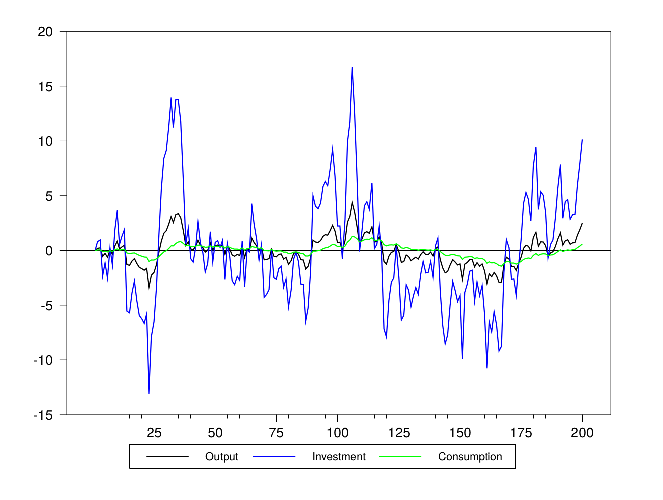
\includegraphics[scale=.9]{rbc1.eps}
  \end{figure}
\end{frame}
%--------------------------------------

%--------------------------------------
\begin{frame}
  RBC's main feature: being able to generate business cycles\\  
\begin{enumerate}
  \item Model roughly matches observed fluctuations in output
  \item Model reflects fact that investment cycles are more volatile than consumption
\end{enumerate}
\end{frame}
%--------------------------------------

%--------------------------------------
\begin{frame}
  \begin{figure}
    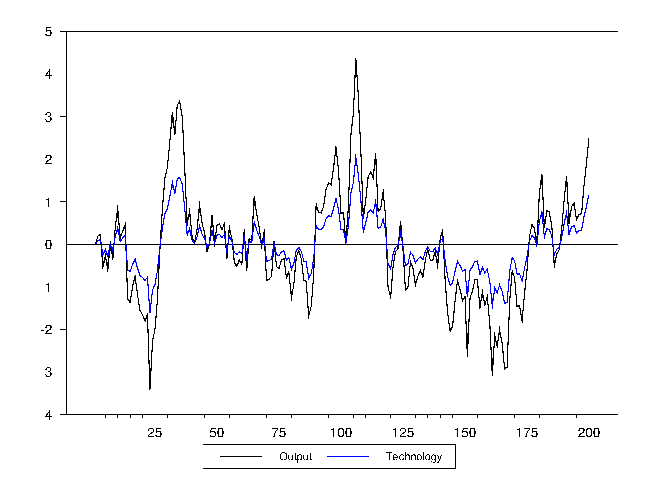
\includegraphics[scale=.9]{rbc2.eps}
  \end{figure}
\end{frame}
%--------------------------------------

%--------------------------------------
\begin{frame}
  \textbf{Technology shocks} relate to business cycles as increases would lead to extra output through
  \begin{enumerate}
    \item Capital accumulation
    \item Inducing people to work more
  \end{enumerate}
  \medskip
  RBC model contains important propagation mechanisms turning technology shocks into business cycles
  \begin{itemize}
    \item In world with identical technology level, RBC model would still generate business cycles
    \item Mechanisms quite weak; output fluctuations follow technology fluctuations quite closely
  \end{itemize}
\end{frame}
%--------------------------------------

%--------------------------------------
\begin{frame}
  \begin{figure}
    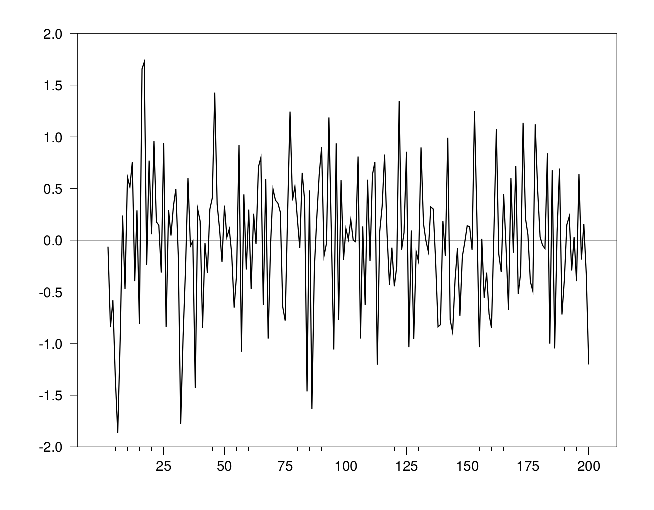
\includegraphics[scale=.9]{rbc3.eps}
  \end{figure}
\end{frame}
%--------------------------------------

%--------------------------------------
\begin{frame}
  Cogley \& Nason (1995) note that RBC models do not match positively autocorrelated growth
  \begin{itemize}
    \item Autocorrelation coefficient is 0.34 in real life
  \end{itemize}
  \medskip
  Authors argue that IRFs need to be hump-shaped
  \begin{itemize}
    \item Growth rate increase followed by another growth rate increase
    \item Reponse to technology shocks do not emulate this
    \item No other source of shocks in model
  \end{itemize}
  \end{frame}
%--------------------------------------

%--------------------------------------
\begin{frame}
  \begin{figure}
    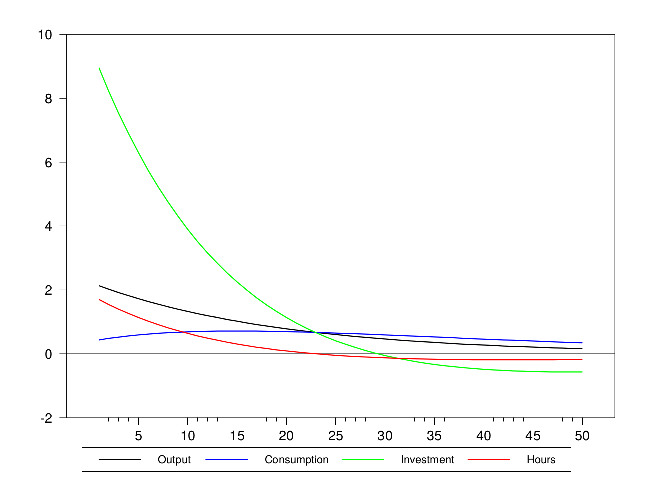
\includegraphics[scale=.9]{rbc4.eps}
  \end{figure}
\end{frame}
%--------------------------------------

%--------------------------------------
\begin{frame}
  \begin{figure}
    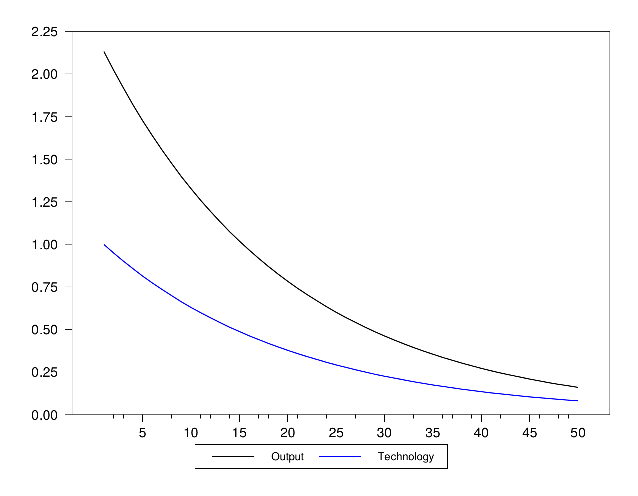
\includegraphics[scale=.9]{rbc5.eps}
  \end{figure}
\end{frame}
%--------------------------------------

%--------------------------------------
\begin{frame}
  \textbf{Extending RBC approach}\\
  Model fails to explain labour market response to technology shocks
  \begin{itemize}
    \item Hours worked tends to decline following positive technology shock
  \end{itemize}
  \medskip
  Fixing deficiencies 
  \begin{enumerate}
    \item Strengthen propagation mechanism
    \begin{itemize}
      \item Adjusting market clearing approach
      \item e.g. lags in investment projects, habit persistence consumer utility
    \end{itemize}
    \medskip
    \item More systematic departure from RBC
    \begin{itemize}
      \item Adding sticky prices/wages
    \end{itemize}
  \end{enumerate}
\end{frame}
%--------------------------------------


%--------------------------------------
\end{document}
